\chapter{An assessment of the potential presented by soft data sources for pluvial flood simulation}
\label{chapter:SoftData}

This thesis has thus far focused on the implementation details for the new computational methods, and evaluating their performance in reproducing known events and standard tests. The previous chapter considered a real-world pluvial event in Newcastle, resulting from a convective storm on 28 June 2012. A limiting factor is the availability of data for such short duration intense events, hence the public were asked to retrospectively contribute photographic evidence, and complete questionnaires, to allow the event to be simulated.

An extensive network exists to monitor river levels and rainfall, consisting pressure transducers, raingauges, and the Met Office's network of C-band radar stations. During progressive fluvial events, this network is invaluable in establishing the relationship between weather and the catchment response, and hence flood consequences. Monitoring is less established in urban environments susceptible to surface water flooding.

Clear evidence also exists that social media is increasingly used as a tool for dissemination and communication during times of crisis and natural disasters, such as during the 2011 Queensland flood and Thai flood \citep{Starbird2010,Vieweg2010,Kongthon2012,Murthy2012}; the accuracy and validity of information provided by the public through social media such as Twitter however may be questionable. A further complication is that only a small portion (approximately 1.5\% but increasing) of Tweets are precisely geotagged \citep{Crampton2013}, which is crucial information for locating and evaluating the extent of flooding. Comparison of locations geocoded from the text within Tweets, against the actual location of the user from geotags, suggests even when Tweets are geotagged, this data can rarely be considered reliable for inferring flooded locations \citep{Leetaru2013}. Clearly, an alternative approach is required.

This chapter considers whether for pluvial flood events, there is scope to use reports from social media to establish flood consequences. A new software framework for integrating these data sources has been developed by the author, described herein. The merit of such an approach, would be capturing reports in near real-time, allowing authorities to prioritise and target their response on those worst affected and most vulnerable.

\section{Background}

\begin{figure*}[tpb]
	\centering
	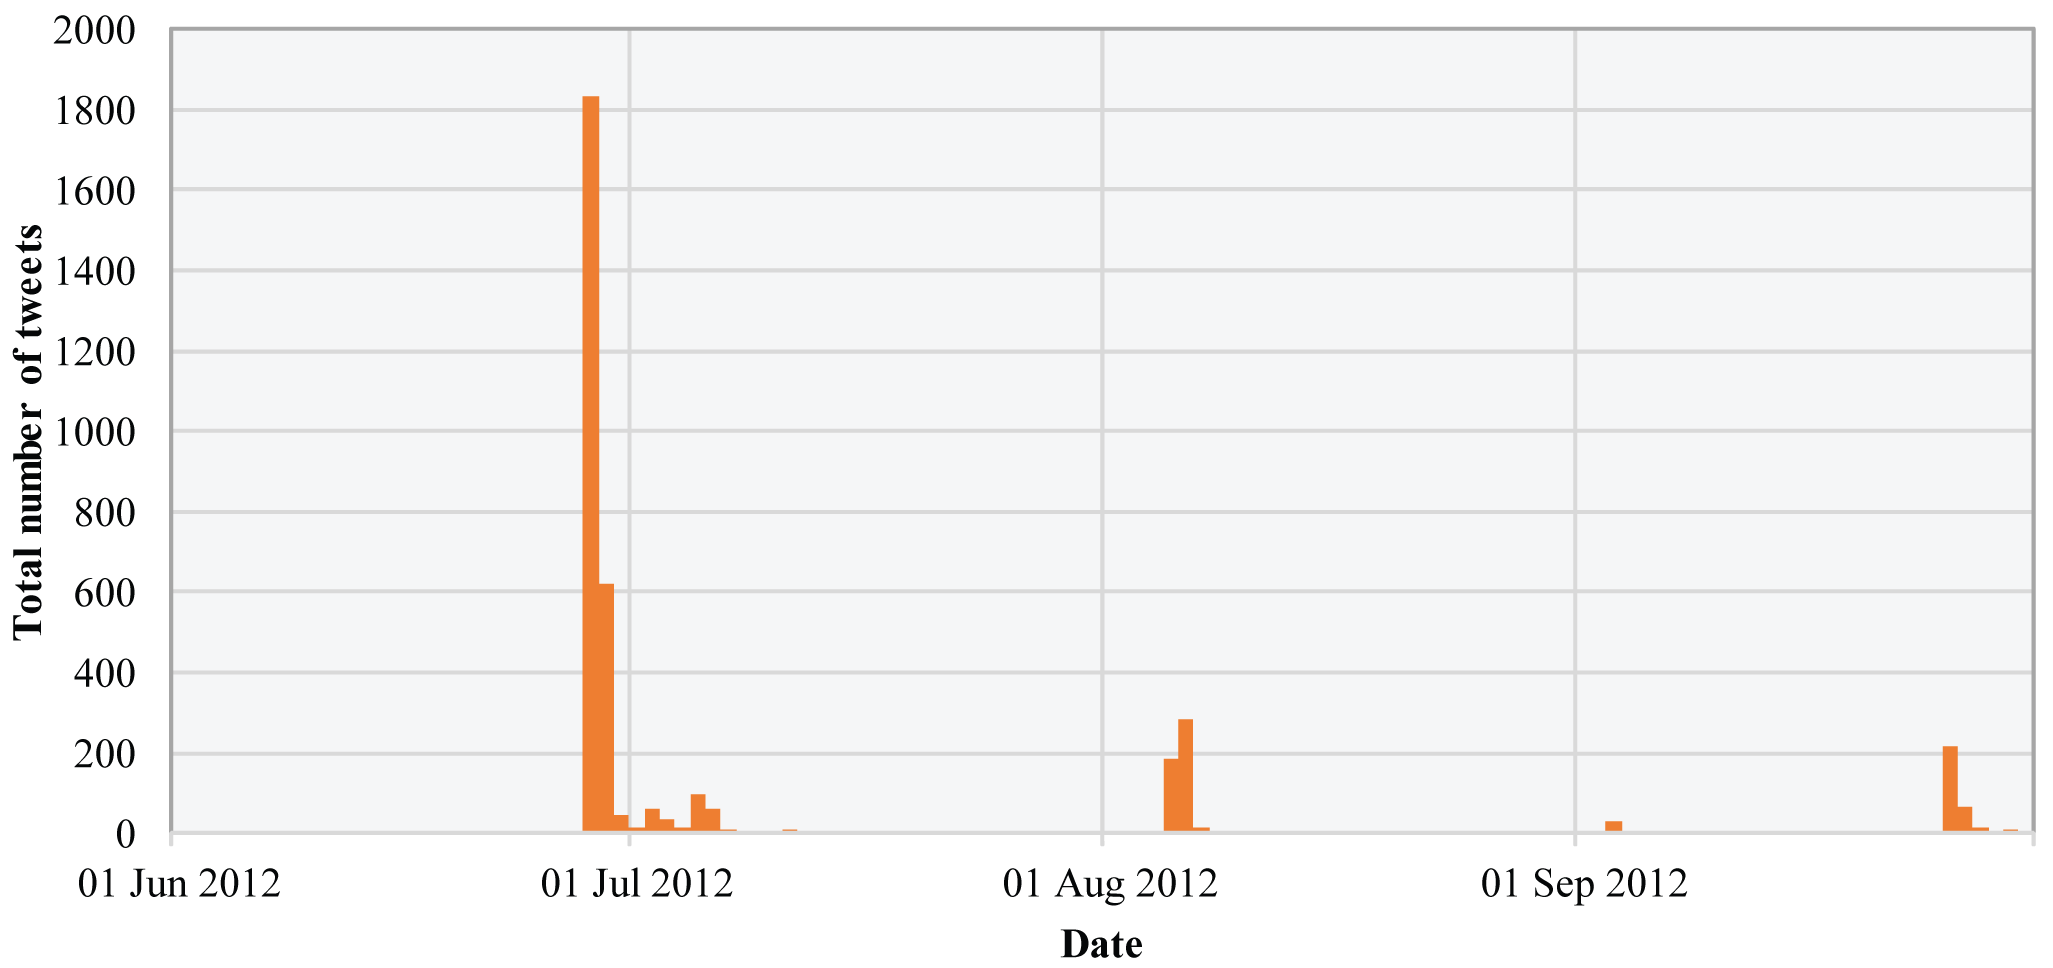
\includegraphics[width=1.0\textwidth]{nowcasting-figures/nclsm-num-tweets.png}
	\caption{Total number of Tweets (including some Retweets) identified about flooding within Tyne and Wear, through hashtags such as \#toonflood and \#newcastleendofdays.}
	\label{NclSM-Num-Tweets}
\end{figure*}

The same flood event from Newcastle is considered. Large numbers of people took to social media to voice their concern, share photos, and find the best way home. Retrospective analysis of Twitter (\url{http://www.twitter.com}) on the day shows more than 1,800 Tweets which could be linked to flooding in the area, helpfully identified by the hashtags \textit{\#toonflood} and \textit{\#newcastleendofdays}. Local authorities and emergency responders both started and actively engaged with these hashtags as a way of disseminating information to the public. A further slightly smaller rainfall event occurred on 5th August 2012, in which 40mm of rainfall fell within 90 minutes \citep{NewcastleCityCouncil2013}. The Twitter activity for these two events is represented in Figure \ref{NclSM-Num-Tweets}, whereby the timing of the August event on a Sunday is believed to be the main reason for the relatively low number of Tweets. 

The same photographic collection used in Chapter \ref{chapter:ScaleEffects} is also considered for validation. Newcastle University asked members of the public to help reconstruct the event through crowd-sourcing, following the success of a similar system following fluvial inundation in nearby Morpeth on 6th September 2008. A simple website allowed photos and text to be uploaded and positioned on a map. The system was publicised through local radio and television, with members of the public encouraged to contribute. 194 submissions were received, almost all including a photo, and the approximate time and location.

\section{Modelling framework}

\begin{figure*}[tpb]
	\centering
	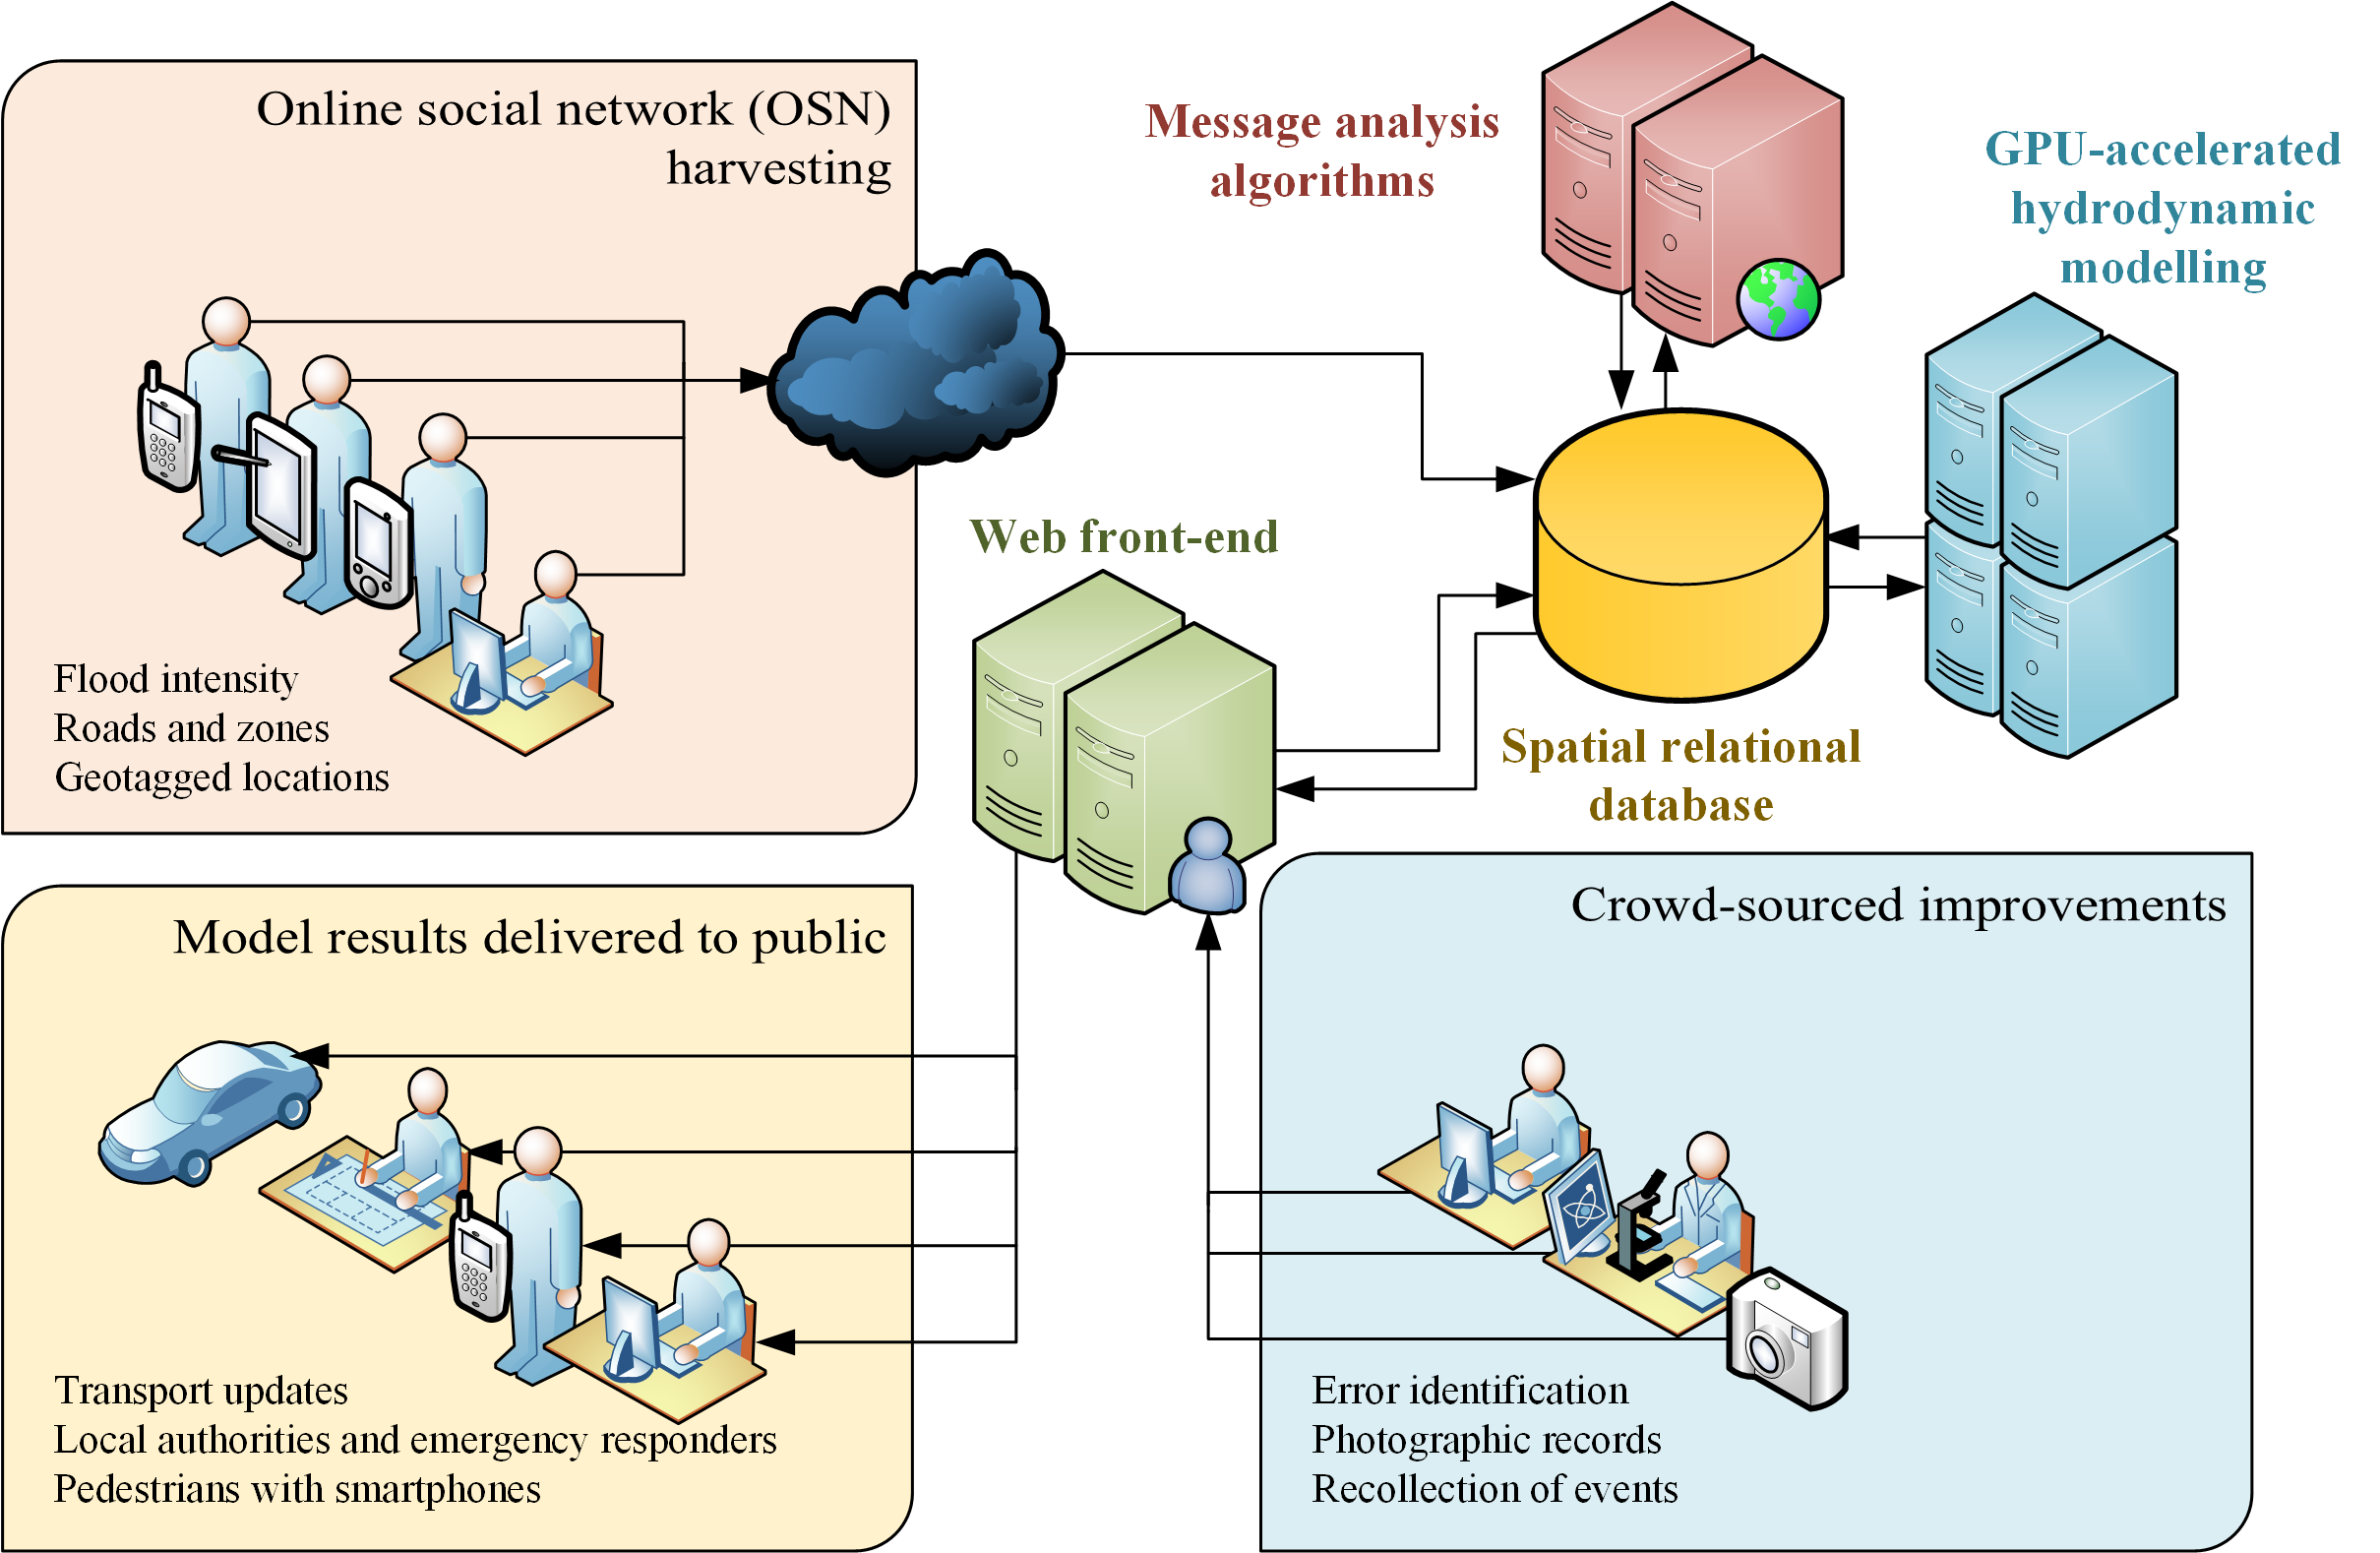
\includegraphics[width=1.0\textwidth]{nowcasting-figures/nclsm-conceptual-diag.png}
	\caption{Conceptual diagram of the integrated real-time modelling framework.}
	\label{NclSM-Conceptual-Diag}
\end{figure*}

The intention is to assess the utility of social networking data and feasibility of real-time high-resolution hydrodynamic modelling, neither of which have previously been explored. Applications of 2D hydraulic models in real-time for surface water flooding are not currently in use within any operational system in the UK \citep{Ghimire2013}. No meteorological data is used in this chapter, and the author is keen to stress that they do not suggest this is the most reliable method for real-time flood inundation modelling. Accordingly, in this framework, the data stream from Twitter is used to identify when a storm event occurs, invoke hydrodynamic model runs in the correct locations, and subsequently validate the quality of results.

The integrated modelling framework takes data from social media, presently only Twitter, and stores messages which may potentially contain valuable data about flooding. These messages are then processed in order to identify criteria against which model runs can be assessed, thereby finding a suitable hydrodynamic model of the flood event, and creating a simulation which closely represents the reported inundation within the city. The results of these simulations can then be fed back to the public and interested parties (e.g. local authorities, emergency responders). Crowd-sourced information including photos and textual descriptions, provide a basis through which future improvements may be made, and the existing system can be validated. The framework is visually represented in Figure \ref{NclSM-Conceptual-Diag}. 

The framework the author has created for this purpose is in effect a Python-based middleware layer, consisting of scripts designed to run as services in the background of a server, mostly remaining idle until a potential flood-causing storm event is identified. Data is stored in a PostgreSQL database with PostGIS extensions for spatial data.

\subsection{Social media harvesting and analysis}

\begin{figure*}[pb]
	\centering
	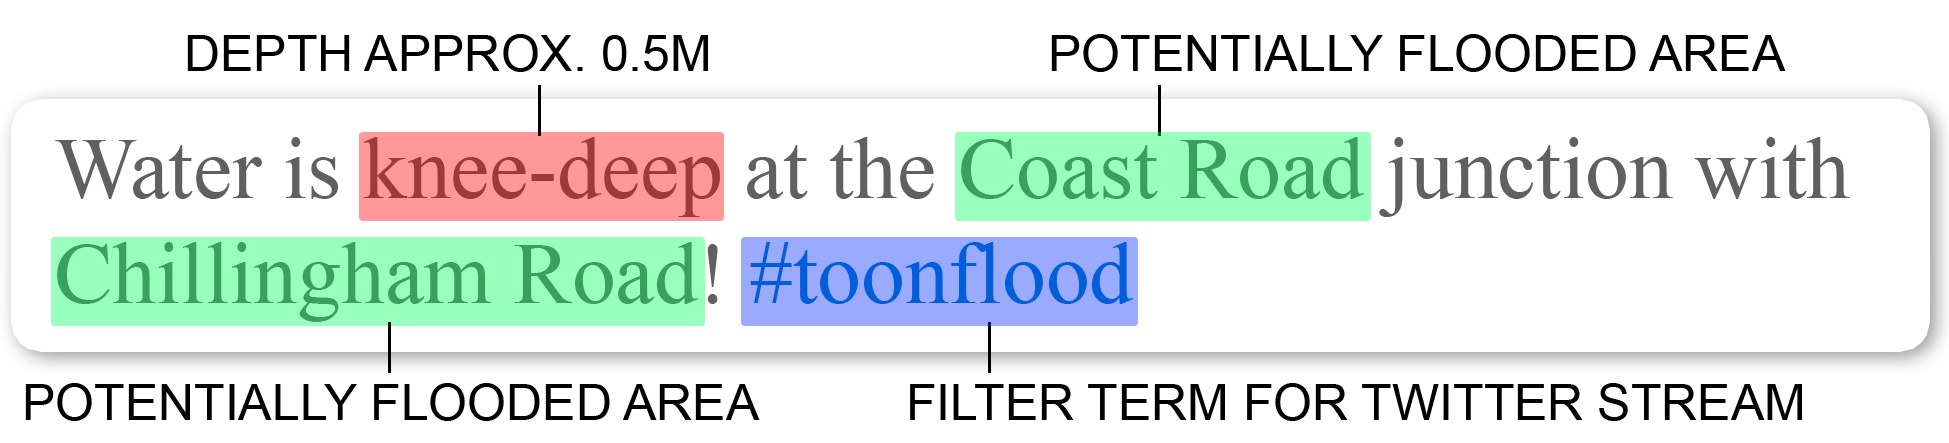
\includegraphics[width=0.8\textwidth]{nowcasting-figures/nclsm-example-tweet.png}
	\caption{An example Tweet (hypothetical) with some of the typical terms that might be identified.}
	\label{NclSM-Example-Tweet}
\end{figure*}

The framework uses a single stream through the Twitter Streaming API, which receives messages filtered both on keywords and spatial extent. The API adopts a broad approach to filtering messages, returning anything which matches any of the criteria; a second round of filtering is therefore carried out before messages are committed to the database. Keywords are matched against phrases or multiple criteria at this point, for example: a Tweet containing the word "flood" with a geotag or bounding box which overlaps with Newcastle; or a Tweet which must match a keyword and a phrase such as ‘flood’ and ‘Newcastle upon Tyne’. 

Criteria are regarded as a conditions against which a model can be assessed, which herein refers to either depth or velocity of flood water; in practice this means a minimum, maximum, or range of values which can be satisfied by the model. For example, `knee-deep' in Figure \ref{NclSM-Example-Tweet} could be satisfied by a depth ranging from 0.3m to 0.8m, acknowledging that people are different heights and the term is only an estimate of the depth. 

In order to comply with the Twitter API terms of service, Tweets including their geoinformation are committed in their entirety to the database, and only held temporarily until they can be analysed, the results of which are anonymous. The temporary storage allows a queue of messages to build pending analysis, which in some instances may take a few seconds for each message.

Analysis of messages focuses on two main areas: identification of terms with potential semantic value for a flood event, and identification of distinct geographic areas. Terms of semantic value are those which potentially indicate the intensity of rainfall, the occurrence of a major storm, the presence of flooding, depth of flooding, or the velocity of flow. Fifty-five terms were initially identified from inspection of messages during previous flood events; notable examples include `black skies', `thunder', `waist deep', and `closed'.  10,217 spatial entities were extracted from a mixture of data sources including Ordnance Survey vector mapping products, OpenStreetMap, and the Royal Mail postcode address file. All of the data used except postcode polygons are freely available in the UK, and no corrections or additions have been made. Accordingly, a similar database could easily be created for any other British urban area. The spatial entities include street names and a large number of building names, allowing messages which refer to flooding in and around markets, parks and shopping centres to be recognised. A hypothetical Tweet has typical terms of interest highlighted in Figure \ref{NclSM-Example-Tweet}.

Once a critical mass of Tweets referring to storm events or rainfall intensity is identified within the database, a storm event is considered to be in progress and the start time assumed to be the same as the first message. Five messages from different users within a fifteen minute period is considered to constitute a `critical mass' herein; however, flood modelling cannot commence until at least one message with a spatial extent and relevant semantic term is identified. A storm event once identified is monitored for a period of four hours, after which it is likely there will be intervention such as pumping in places of strategic importance, although this period can be reconfigured to be longer. It is assumed the intense rainfall will last for no longer than an hour for the purposes of simulations with a standardised event. These numbers are appropriate for the short duration heavy rainfall induced flooding which typically occurs in summer in the UK; the framework is not suitable for use with groundwater or fluvial inundation events.

\subsection{Real-time modelling}

\begin{figure*}[tpb]
	\centering
	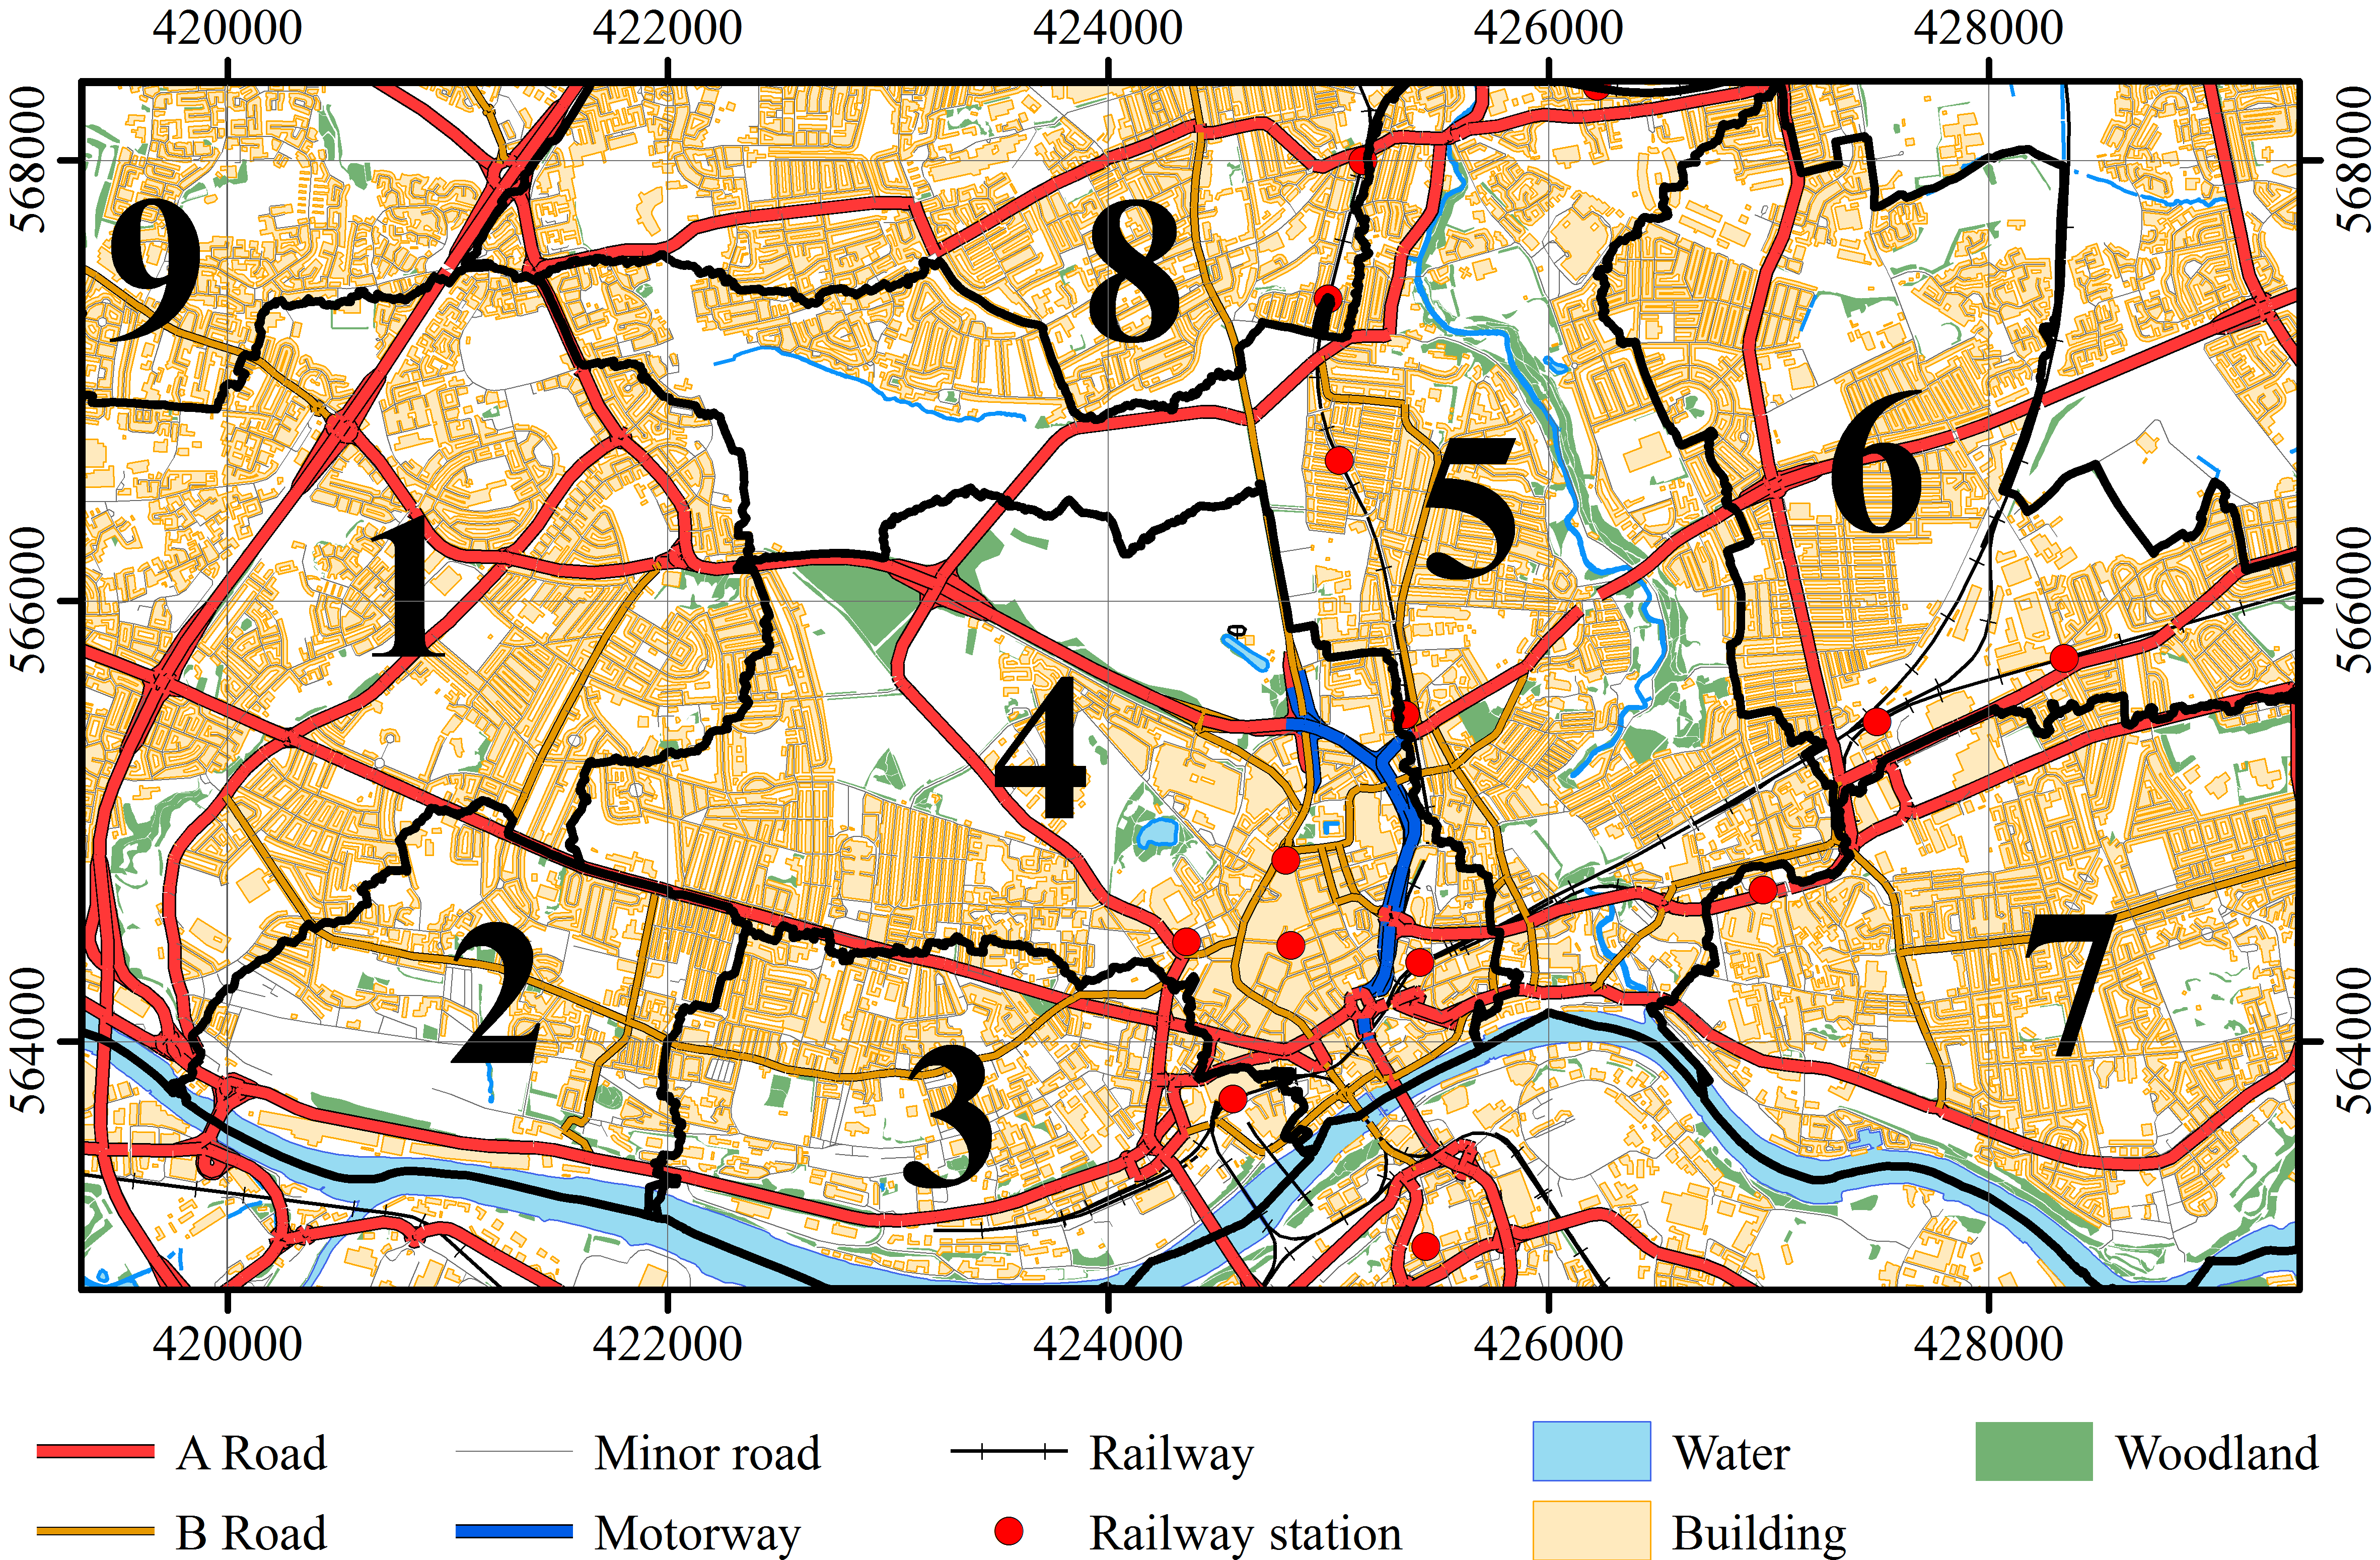
\includegraphics[width=1.0\textwidth]{nowcasting-figures/nclsm-map-models.png}
	\caption{Map showing the nine different models for Newcastle upon Tyne used in the social media framework.}
	\floatfoot{Contains Ordnance Survey data \copyright{} Crown copyright and database right 2013.}
	\label{NclSM-Map-Models}
\end{figure*}

Airborne altimetric LiDAR data is used to represent the topography of the city for hydrodynamic modelling. A digital elevation model (DEM) was created by the extraction and superposition of walls and buildings from the raw LiDAR data to a post-processed terrain model resulting from the same dataset. Both the raw and post-processed data is readily and commercially available at low cost, and allows for a model of the city topography free of artefacts, without bridges and trees, but including barriers to flow (e.g. walls). A grid resolution of 2m was selected to ensure the timely completion of simulations, whilst still clearly representing the majority of smaller flow pathways (i.e. gaps between buildings, alleyways, etc.).

Simulations are constrained to the area shown in Figure \ref{NclSM-Map-Models}, which excludes the more rural areas to the north of the city. Analysis of the topography identified watersheds and allowed the city to be split to form nine different models, all with transmissive boundary conditions but no flow exchanged between them. Only the area under the remit of Newcastle City Council is modelled. The areas covered by each model are also shown in Figure \ref{NclSM-Map-Models}.

For clarity, this approach differs from the domain decomposition methods outlined in Chapter \ref{chapter:Decomposition}, because pluvial flooding may affect a small area of the city, given the spatial concentration of convective storms. A number of smaller discrete models is hence adopted. A potential future alternative would be dynamically generating a model from the extent of the social media records, and performing domain decomposition on this.

The drainage network and associated sewers are not explicitly considered within the model, owing partly to a lack of suitable data regarding the grates and gullies, and more crucially because its effects and quality of operation during an extreme rainfall are likely to be minimal. Nevertheless in the event of small amounts of rainfall, this would be adequately removed by the drainage network; accordingly, a very simple approximation is implemented, for losses at a rate of 12.5mm/hr in all cells, consistent with the previous chapter.

\begin{figure*}[tpb]
	\centering
	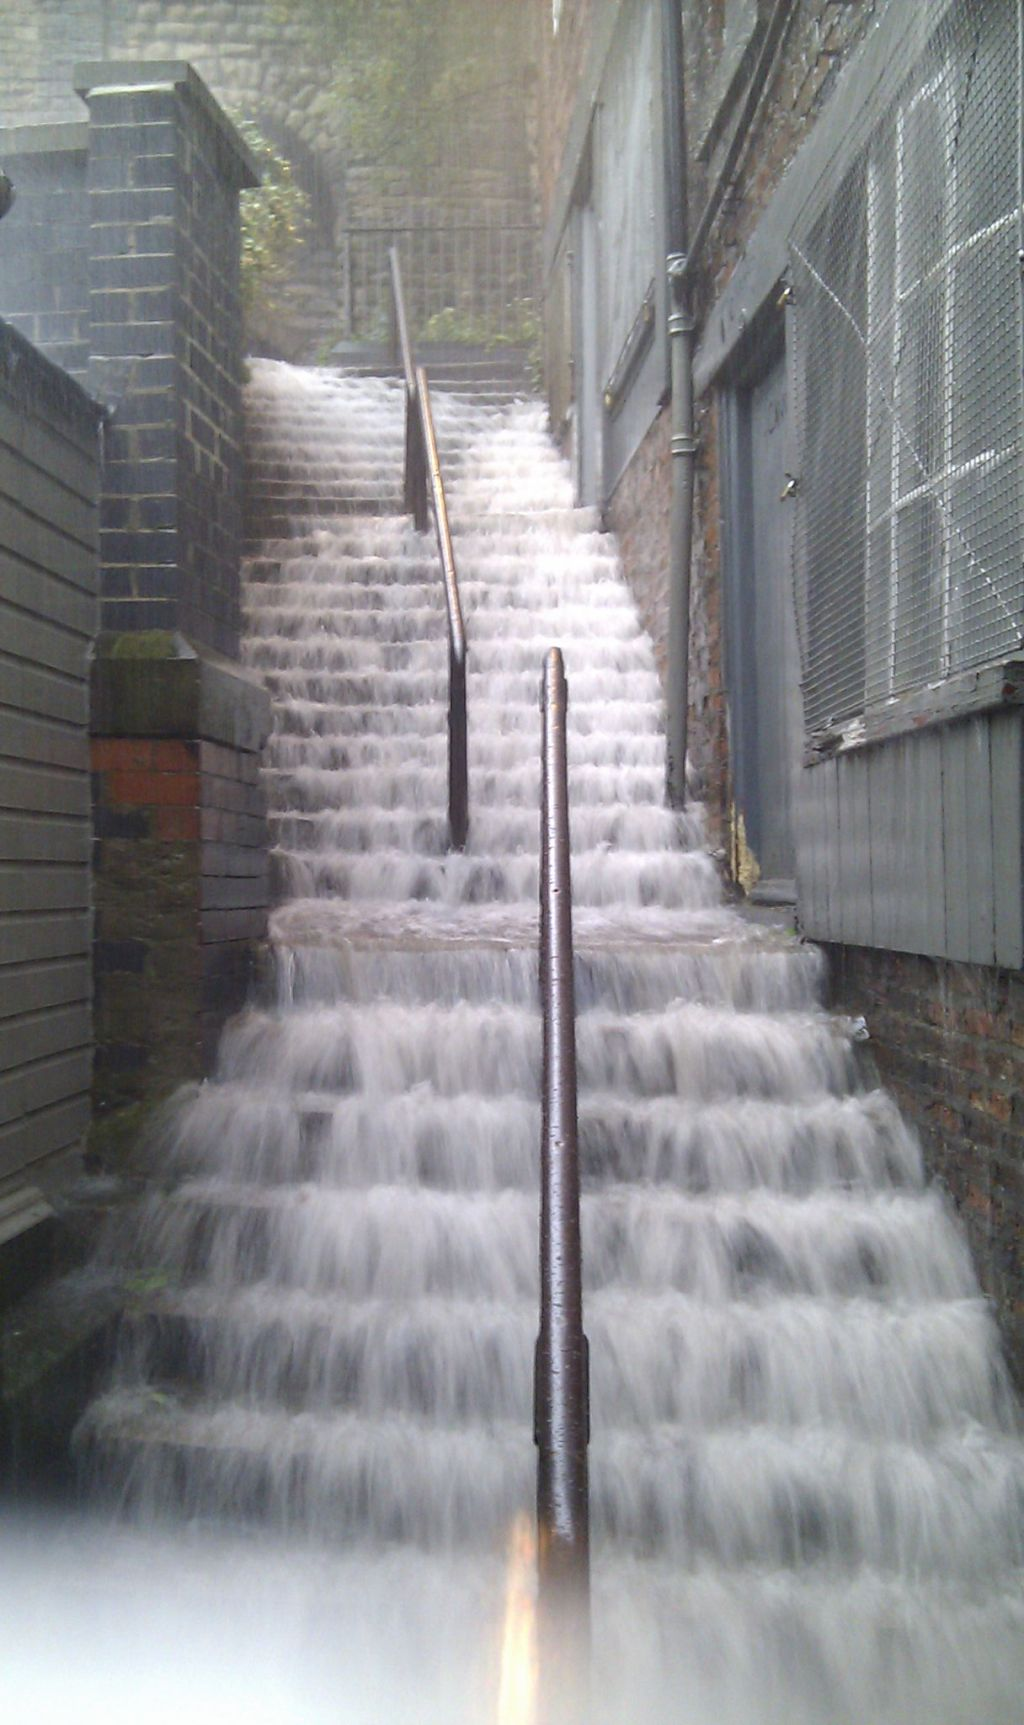
\includegraphics[width=0.4\textwidth]{nowcasting-figures/nclsm-example-supercritical.jpg}
	\caption{An example of the complex and dangerous hydrodynamics which can occur in urban flooding, showing water cascading at high speeds down steep steps in Newcastle upon Tyne.}
	\label{NclSM-Example-Supercritical}
\end{figure*}

A uniform Manning coefficient across the domain is assumed to be $0.045 s m^{-1/3}$ to partially compensate for street furniture which is neglected, and the mixture of surfaces which include long grass and woodland, paving stones, and asphalt. A basic sensitivity analysis suggested minimal effect for this simulation from variations in the Manning coefficient. Simulations are for a two-hour period, whilst rainfall is applied uniformly across the domain for one hour. This allows the rainfall to settle. The shape of the hyetograph for an actual event may of course be significant, perhaps concentrating the heaviest rainfall within a 5-minute window, but it is not feasible (or in the author's opinion, possible without a large volume of data) to establish this from social media. 

Evidence obtained from crowd-sourced images of the June flooding demonstrably confirmed expectations that high velocity and complex flow conditions would be present in parts of the city, such as where flow cascaded down steps, and hydraulic jumps forming on steep roads (e.g. Figure \ref{NclSM-Example-Supercritical}). Reproduction of these effects requires a shock-capturing model. Efficient and expedient simulation of a 48km$^2$ area with almost 12 million cells for real-time flood simulation is beyond the capabilities of most shock-capturing hydraulic models, which are extremely computationally intensive. The same software described in Chapter \ref{chapter:NumericalMethods} is applied here, without any decomposition. The 2m resolution selected herein nonetheless has limitations, such as the stairs shown in Figure \ref{NclSM-Example-Supercritical} which do not align with the Cartesian grid and are not captured at this resolution; furthermore, this would in effect be considered as a single steep slope within the model rather than individual steps, for which the hydrodynamic behaviour is different.

Chapters \ref{chapter:NumericalValidation} and \ref{chapter:Decomposition} demonstrate that a significant speed-up can be achieved for shock-capturing hydrodynamic simulations using modern GPUs designed for use in scientific computing. Four NVIDIA Tesla M2075 GPUs are used to execute simulations, with a simple database-driven system generating model configurations, monitoring performance, queuing, and dispatching further runs required. Typical simulation run-times are given in Table \ref{NclSM-Performance}, although minor variations can be expected for different rainfall intensities and Manning coefficients. Further experiments conducted confirm that using domain decomposition rather than individual models, it is possible to reduce the runtime for all of the areas given in Table \ref{NclSM-Performance} within a single model to an hour, although this required considerable computing resources (eight scientific-grade GPUs); with access to further resources these runtimes could be further reduced. This technique is not applied herein as some parts of the city had very little social media activity during the events, thus only a subset of models were required. Whilst it is possible to simulate the flooding at more than twice real-time speed, even these reduced runtimes would still be a limiting factor in applications for forecasting. This chapter therefore focuses on the utility of social media for nowcasting and incident management.

\begin{table*}[tpb]
	\newcolumntype{R}[1]{>{\RaggedLeft\arraybackslash}p{#1}}
	\small
	\centering
	\caption{Run-times and descriptions for the different models used to simulate flooding in Newcastle upon Tyne.}
	\label{NclSM-Performance}
	\begin{tabular}{p{0.1\textwidth}p{0.2\textwidth}R{0.15\textwidth}R{0.15\textwidth}R{0.15\textwidth}}
		\toprule
		\raggedright{Model ID} & \raggedright{Model description} & Area (km$^2$) & Cell count & Run-time (hh:mm:ss) \\
		\midrule
		1	&	Fenham		&	7.39	&	1,847,500	&	00:32:08	\\
		2	&	Elswick west	&	2.98	&	745,000	&	00:13:08	\\
		3	&	Elswick east	&	3.74	&	935,000	&	00:17:24	\\
		4	&	City centre		&	7.01	&	1,752,500	&	00:30:10	\\
		5	&	Ouseburn		&	9.29	&	2,322,500	&	00:43:56	\\
		6	&	Heaton		&	5.28	&	1,320,000	&	00:20:25	\\
		7	&	Walker		&	5.67	&	1,417,500	&	00:17:44	\\
		8	&	Gosforth		&	4.06	&	1,015,000	&	00:13:37	\\
		9	&	Westerhope	&	2.31	&	577,500	&	00:07:04	\\
		\bottomrule
	\end{tabular}
\end{table*}

Results from simulations are stored to raster files at 450 second intervals in the simulation. These include the current depth, maximum depth recorded in a cell, and the velocity in the $x-$ and $y-$ Cartesian directions. These result files are subsequently analysed to determine if a simulation is matching the criteria identified from social media. Each simulation runs only to the next 450 second interval while the event is in progress, and only models where suitable criteria were identified from social media are scheduled for execution; this means that even though multiple model runs are required to find an appropriate match, these can often be achieved in near real-time.

\subsection{Flood model result analysis}

Resultant raster files are analysed for each criterion identified using social media. These criteria stipulate that the depth or velocity in a geographic area should either exceed a value or fall within a defined range. A large number of messages identified, referred to a spatial location by describing a nearby landmark or intersection, such as a road being closed at the junction with another, or flooding occurring near to a named shopping centre. Spatial entities are therefore buffered to create an area to extract from the output raster files; the example in Figure \ref{NclSM-Example-Buffer} shows a leisure complex with a 75m buffer area around it, and the flooding referred to in numerous Tweets can clearly be seen approximately 50 to 100m away. The size of the buffer is configurable. The section of road missing from the buffered area in the figure also shows one of the minor issues with the approach adopted, whereby some spatial features lie close to or on the boundary between the nine different models; in such cases multiple result files must be consulted.

Each cell within the buffered area is used to generate a histogram for the variable under consideration, an example of which is given in Figure \ref{NclSM-Example-Histogram}, where a typical shape is exhibited with the majority of cells effectively dry. The larger depths are therefore of more interest in determining whether an area is flooded; however, taking the maximum value would potentially identify exceptional cells that are a consequence of deficiencies or artefacts in the terrain model. For the results presented herein, a range of 0.01 to 5.01m is used for depth histograms, and 0.01 to 1.01ms$^-1$ for velocity, in both cases with 500 bins. The approach adopted uses the histogram to obtain approximations (which are fairly accurate given the bin size) for the 70th and 95th percentile values, and considers a criterion to be satisfied if there is an overlap between the criterion and the range between these percentiles. The percentile range used is also configurable. In the event that multiple criteria arise from a single Tweet, for example if the words ‘flooded’ and ‘knee-deep’ were found, then only the most stringent criterion will be considered (i.e. knee-deep).

\begin{figure*}[tpb]
	\centering
	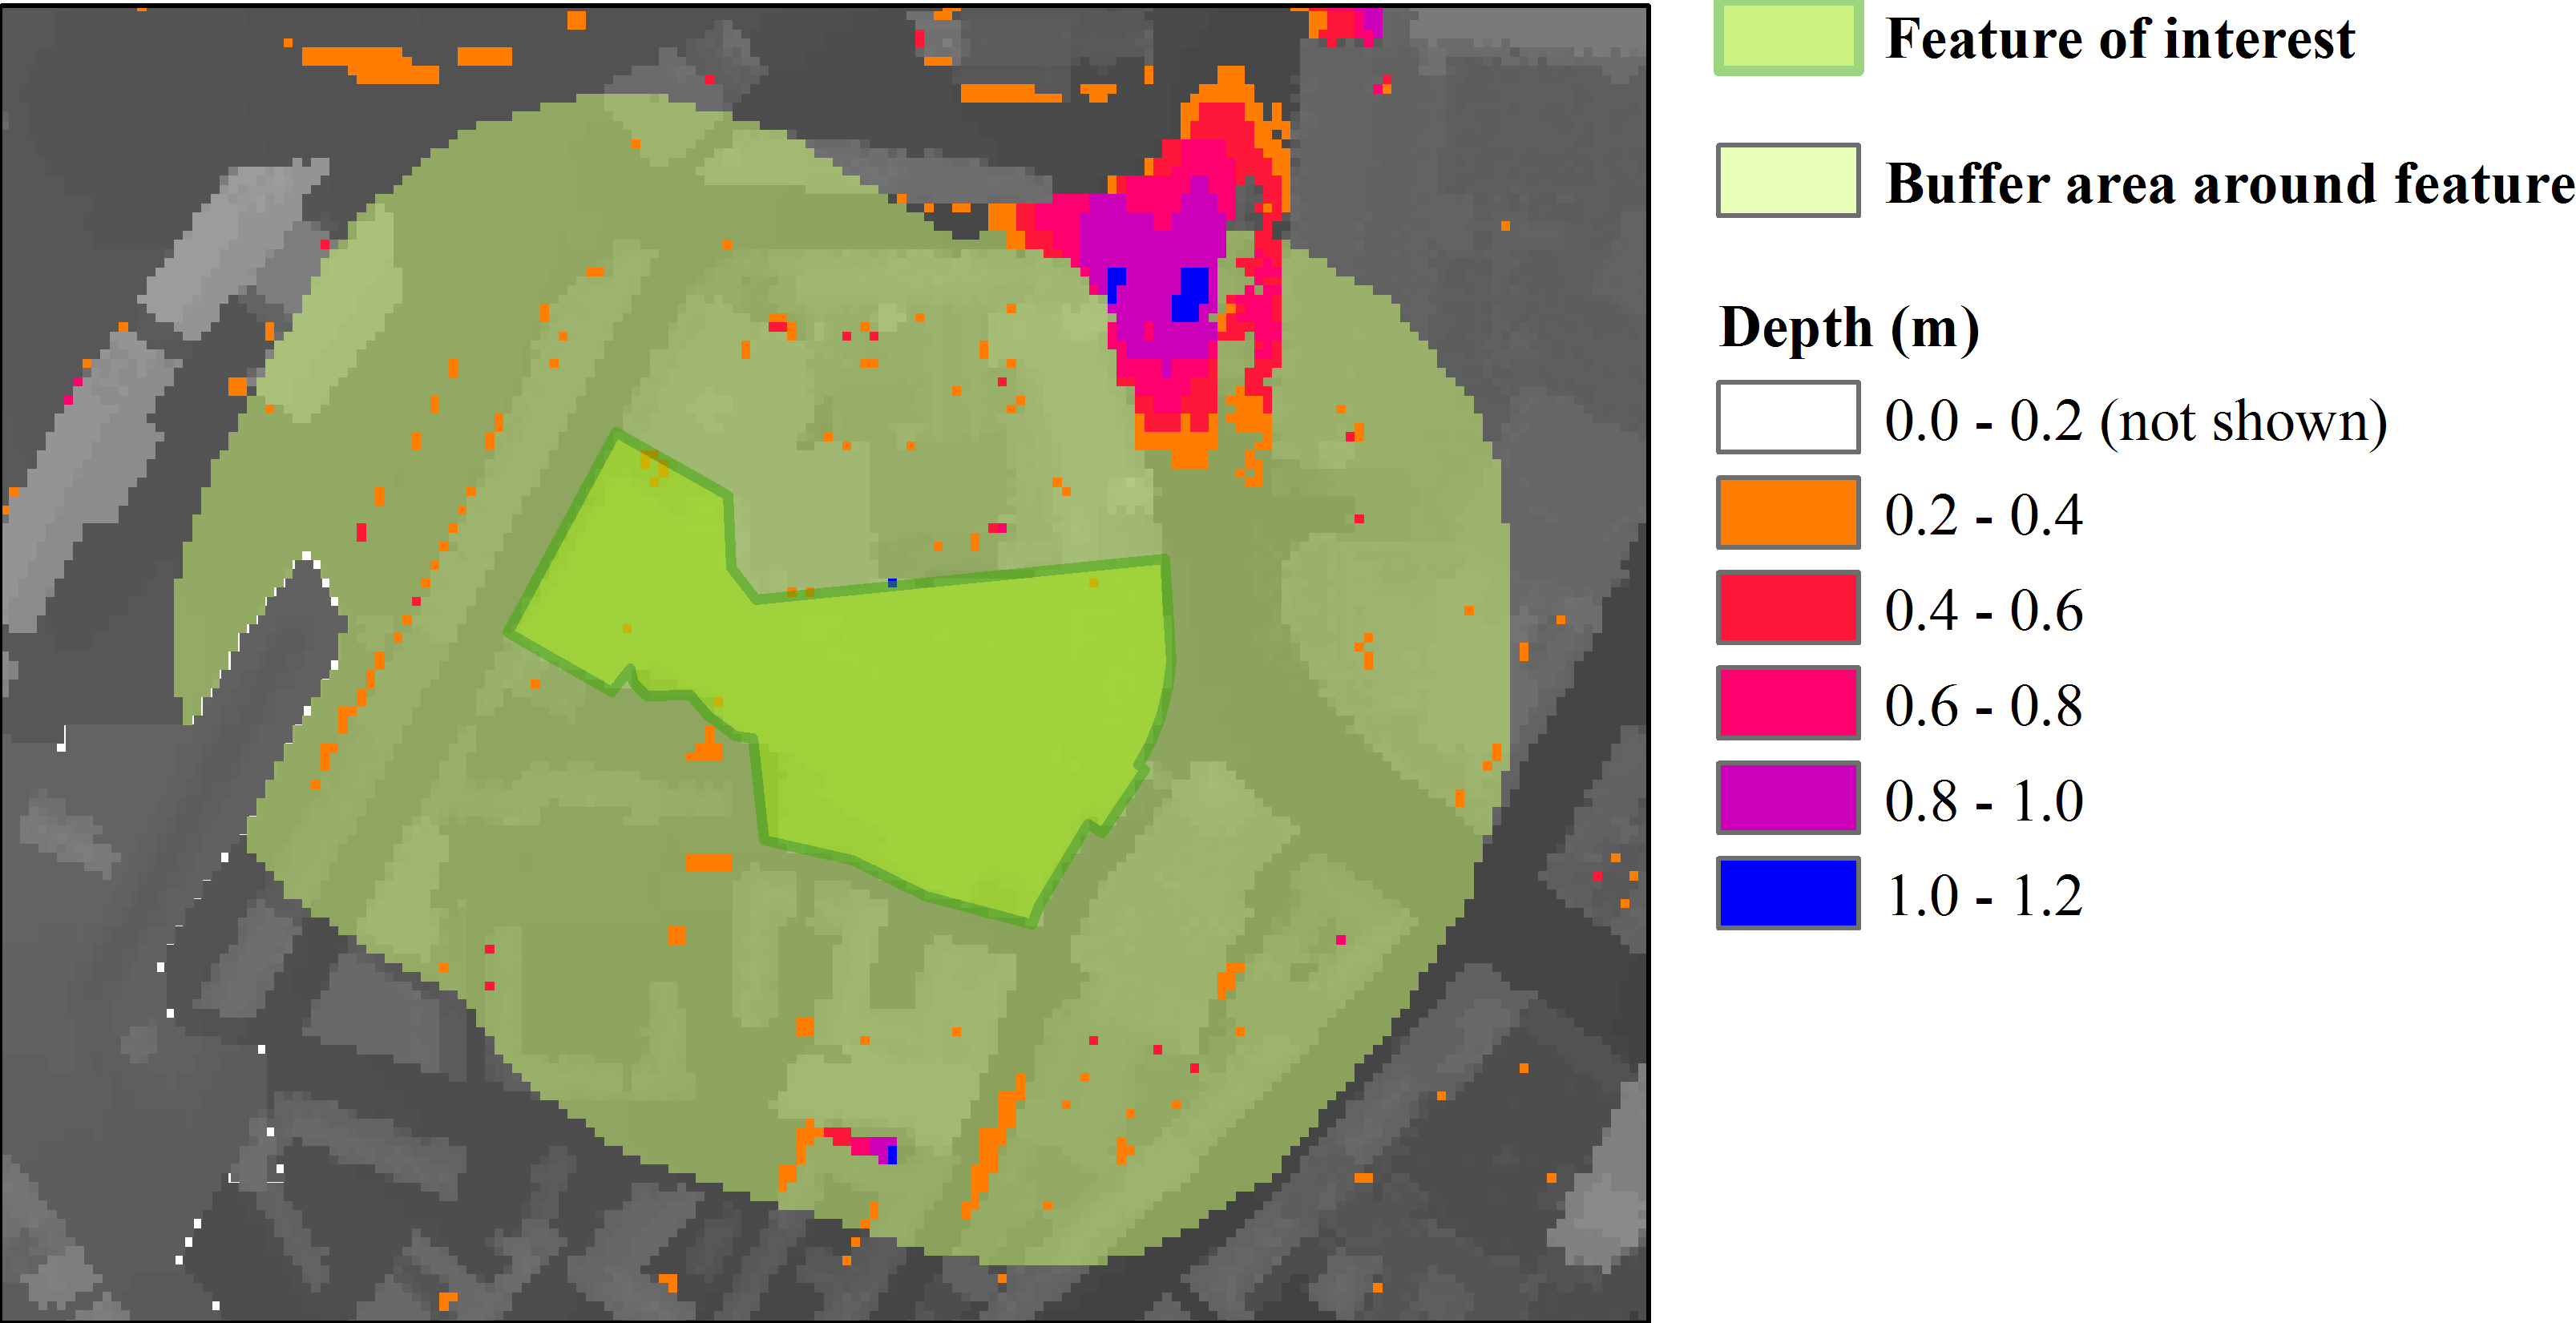
\includegraphics[width=1.0\textwidth]{nowcasting-figures/nclsm-example-buffer.png}
	\caption{An example 75m buffered area used to check whether a model has satisfied a depth criterion surrounding a leisure complex.}
	\label{NclSM-Example-Buffer}
\end{figure*}

\begin{figure*}[tpb]
	\centering
	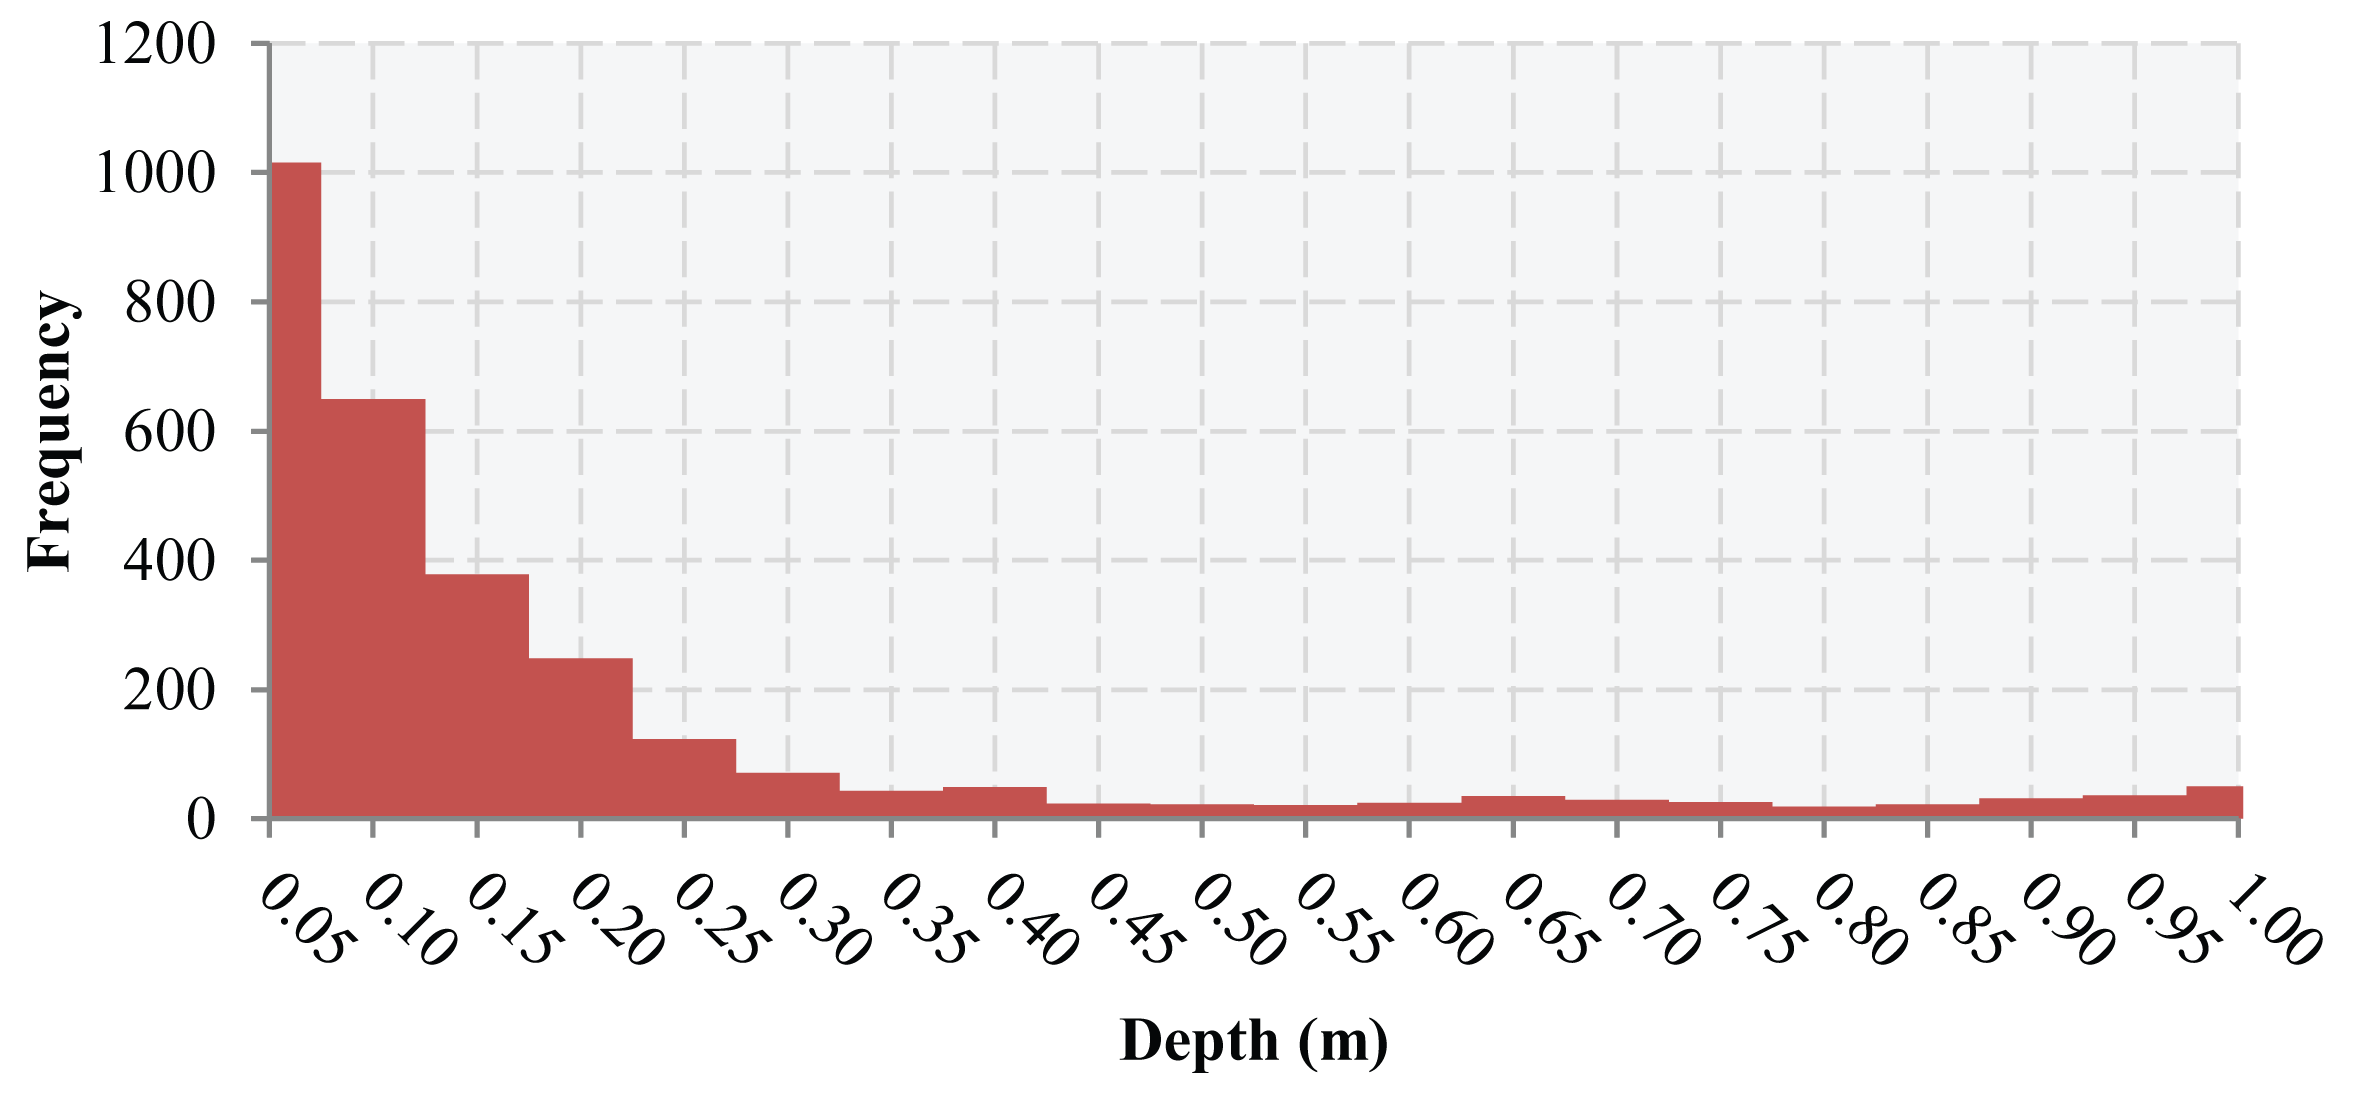
\includegraphics[width=1.0\textwidth]{nowcasting-figures/nclsm-example-histogram.png}
	\caption{An example histogram produced from the depth in cells surrounding the feature in Figure \ref{NclSM-Example-Buffer}.}
	\label{NclSM-Example-Histogram}
\end{figure*}

The modelling framework is designed to use known or suspected data about flooding in one part of the city to infer areas elsewhere which might be flooded, as a consequence of the same rainfall event. It is therefore not crucial that the framework correctly identifies the amount of rainfall, especially given how spatially varied this could be, but instead identifies a single simulation which best matches social media data. Identification of the best result set is therefore taken to be the lowest amount of rainfall which satisfies the majority of criteria, where the improvement achieved by adding a further 5mm of rainfall is less than 5\% of the criteria. The gradient of criteria satisfied against total rainfall volume is the key determinant. Whilst ideally the number of criteria satisfied might be expected to eventually begin to decrease with excessive amounts of rainfall, this is often not the case, as the majority of criteria only stipulate a minimum depth (i.e. knowing somewhere has been closed or flooded, results in a criteria based only on minimum depth). 

\section{Results and discussion}

The integrated modelling framework was tested using retrospective data collected from Twitter following the two major flood events in Newcastle upon Tyne during 2012, the smaller of the two occurring on 5th August and the larger on 28th June. For the two events respectively, a total of 186 and 1,834 Tweets were collected; however, only 168 and 1,243 of these were within four hours of the framework identifying a potential event in progress.

The event on 28th June is believed to have spread 50mm of rainfall over some parts of the city, with peak rainfall rates approaching 200mm/hr. Analysis of UK Met Office NIMROD rainfall radar for the event suggests the average across the city was approximately 46mm. The 5th August event by contrast is thought to have totalled 30-40mm. The framework makes no accommodation for spatial variations in rainfall rate, the varying intensity, and uses only a simple assumption for drainage losses. For simulations hereafter, 10mm and 80mm events were completed in advance, providing a starting point for the framework to begin new model runs. 

\subsection{Geolocating Tweets and identifying binary assertions against which to assess model performance}

From the aforementioned Tweets with timestamps in the first four hours of each event, semantically relevant terms and spatial location names were matched. Those with both present, where the semantic term infers implications for either a depth or velocity, are considered to be useful. Only 43 such Tweets could be identified for 28th June, and 13 for 5th August, shown in Figure \ref{NclSM-Tweet-Breakdown}. On 28th June, the first Tweet about the weather was made at 15:57, whilst the first Tweet with enough detail to create a model criterion was at 16:12. On 5th August the first tweet was at 13:44, but a whole hour later before a Tweet containing enough data for a model criterion, which is a prohibitively long time in terms of incident management.

Manual inspection of Tweets will clearly identify further useful information; however, the framework is intended to be completely automated; consequently, some instances where typing errors were made or colloquial terms used to refer to areas resulted in no match. Implementation of the Levenshtein algorithm, Soundex, or vernacular geographies for geocoding could assist and may be explored in the future. Geotagged Tweets identified during both events were not found to be of practical use; in some instances the geotag identified a location different to where flooding was occurring, often in the case of Retweets. 

\begin{figure*}[tpb]
	\centering
	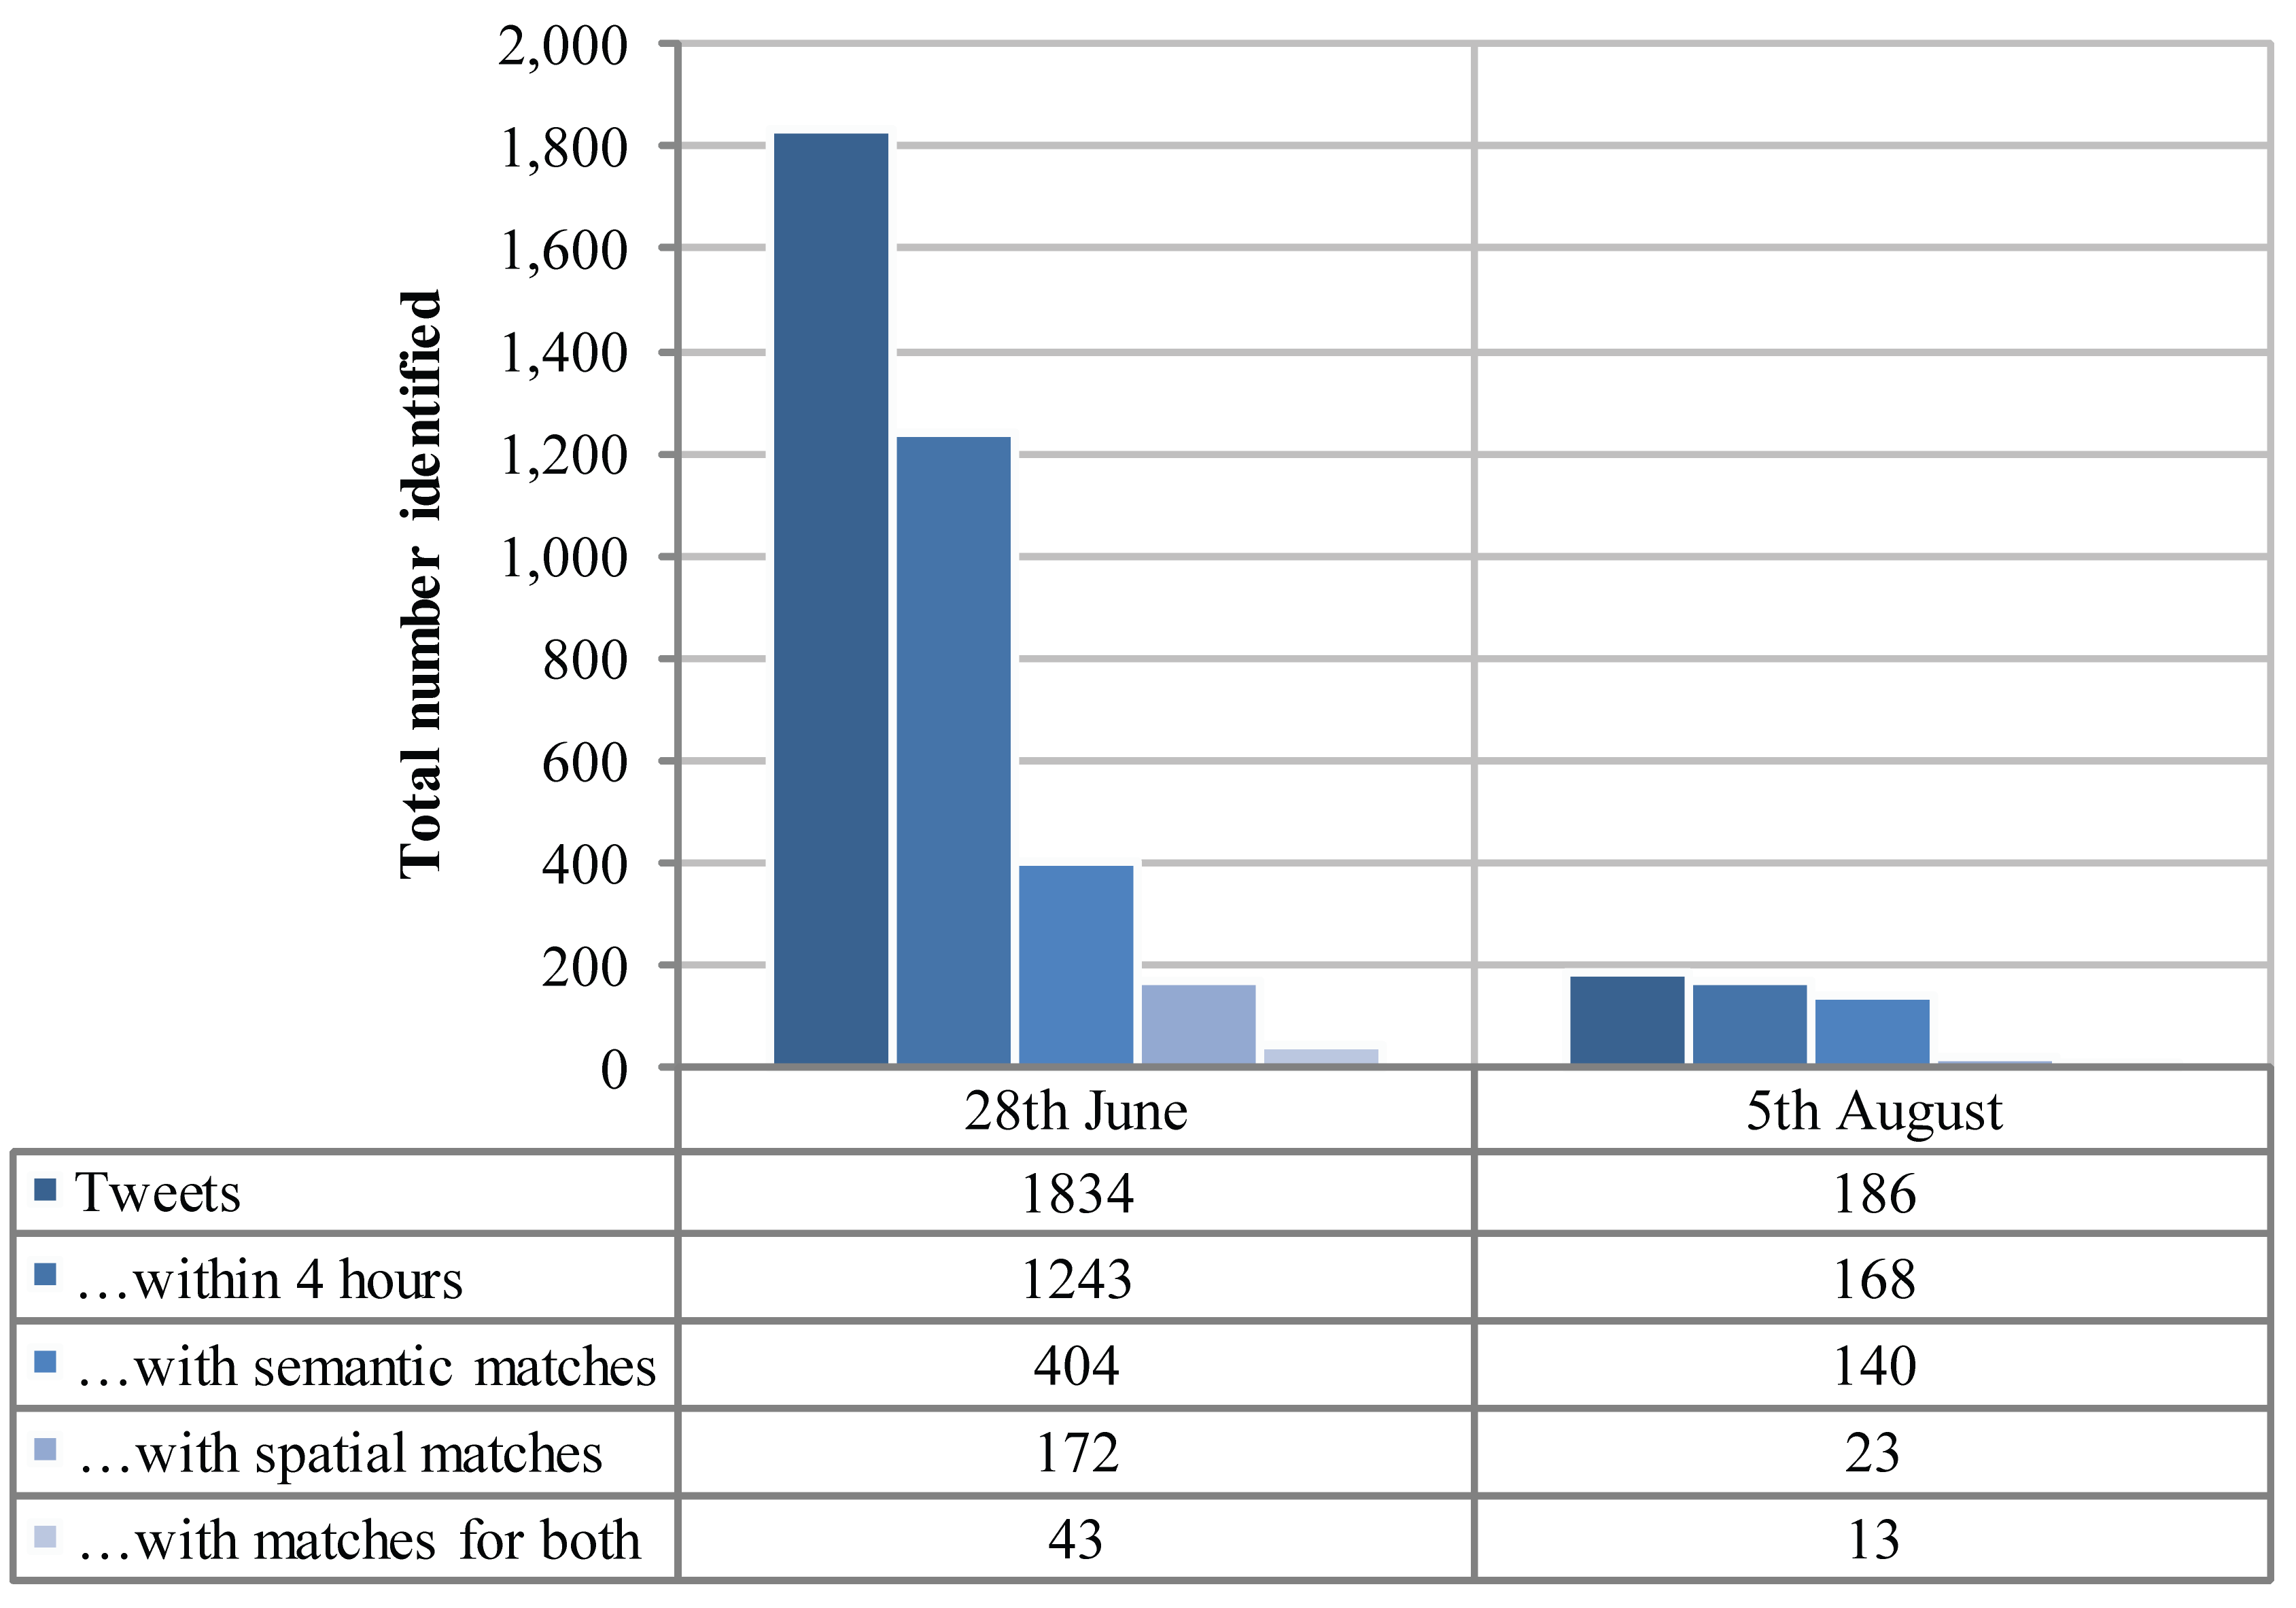
\includegraphics[width=1.0\textwidth]{nowcasting-figures/nclsm-tweet-breakdown.png}
	\caption{Number of useful Tweets identified and how many of these could be used as criteria to assess models against.}
	\label{NclSM-Tweet-Breakdown}
\end{figure*}

\begin{figure*}[tpb]
	\centering
	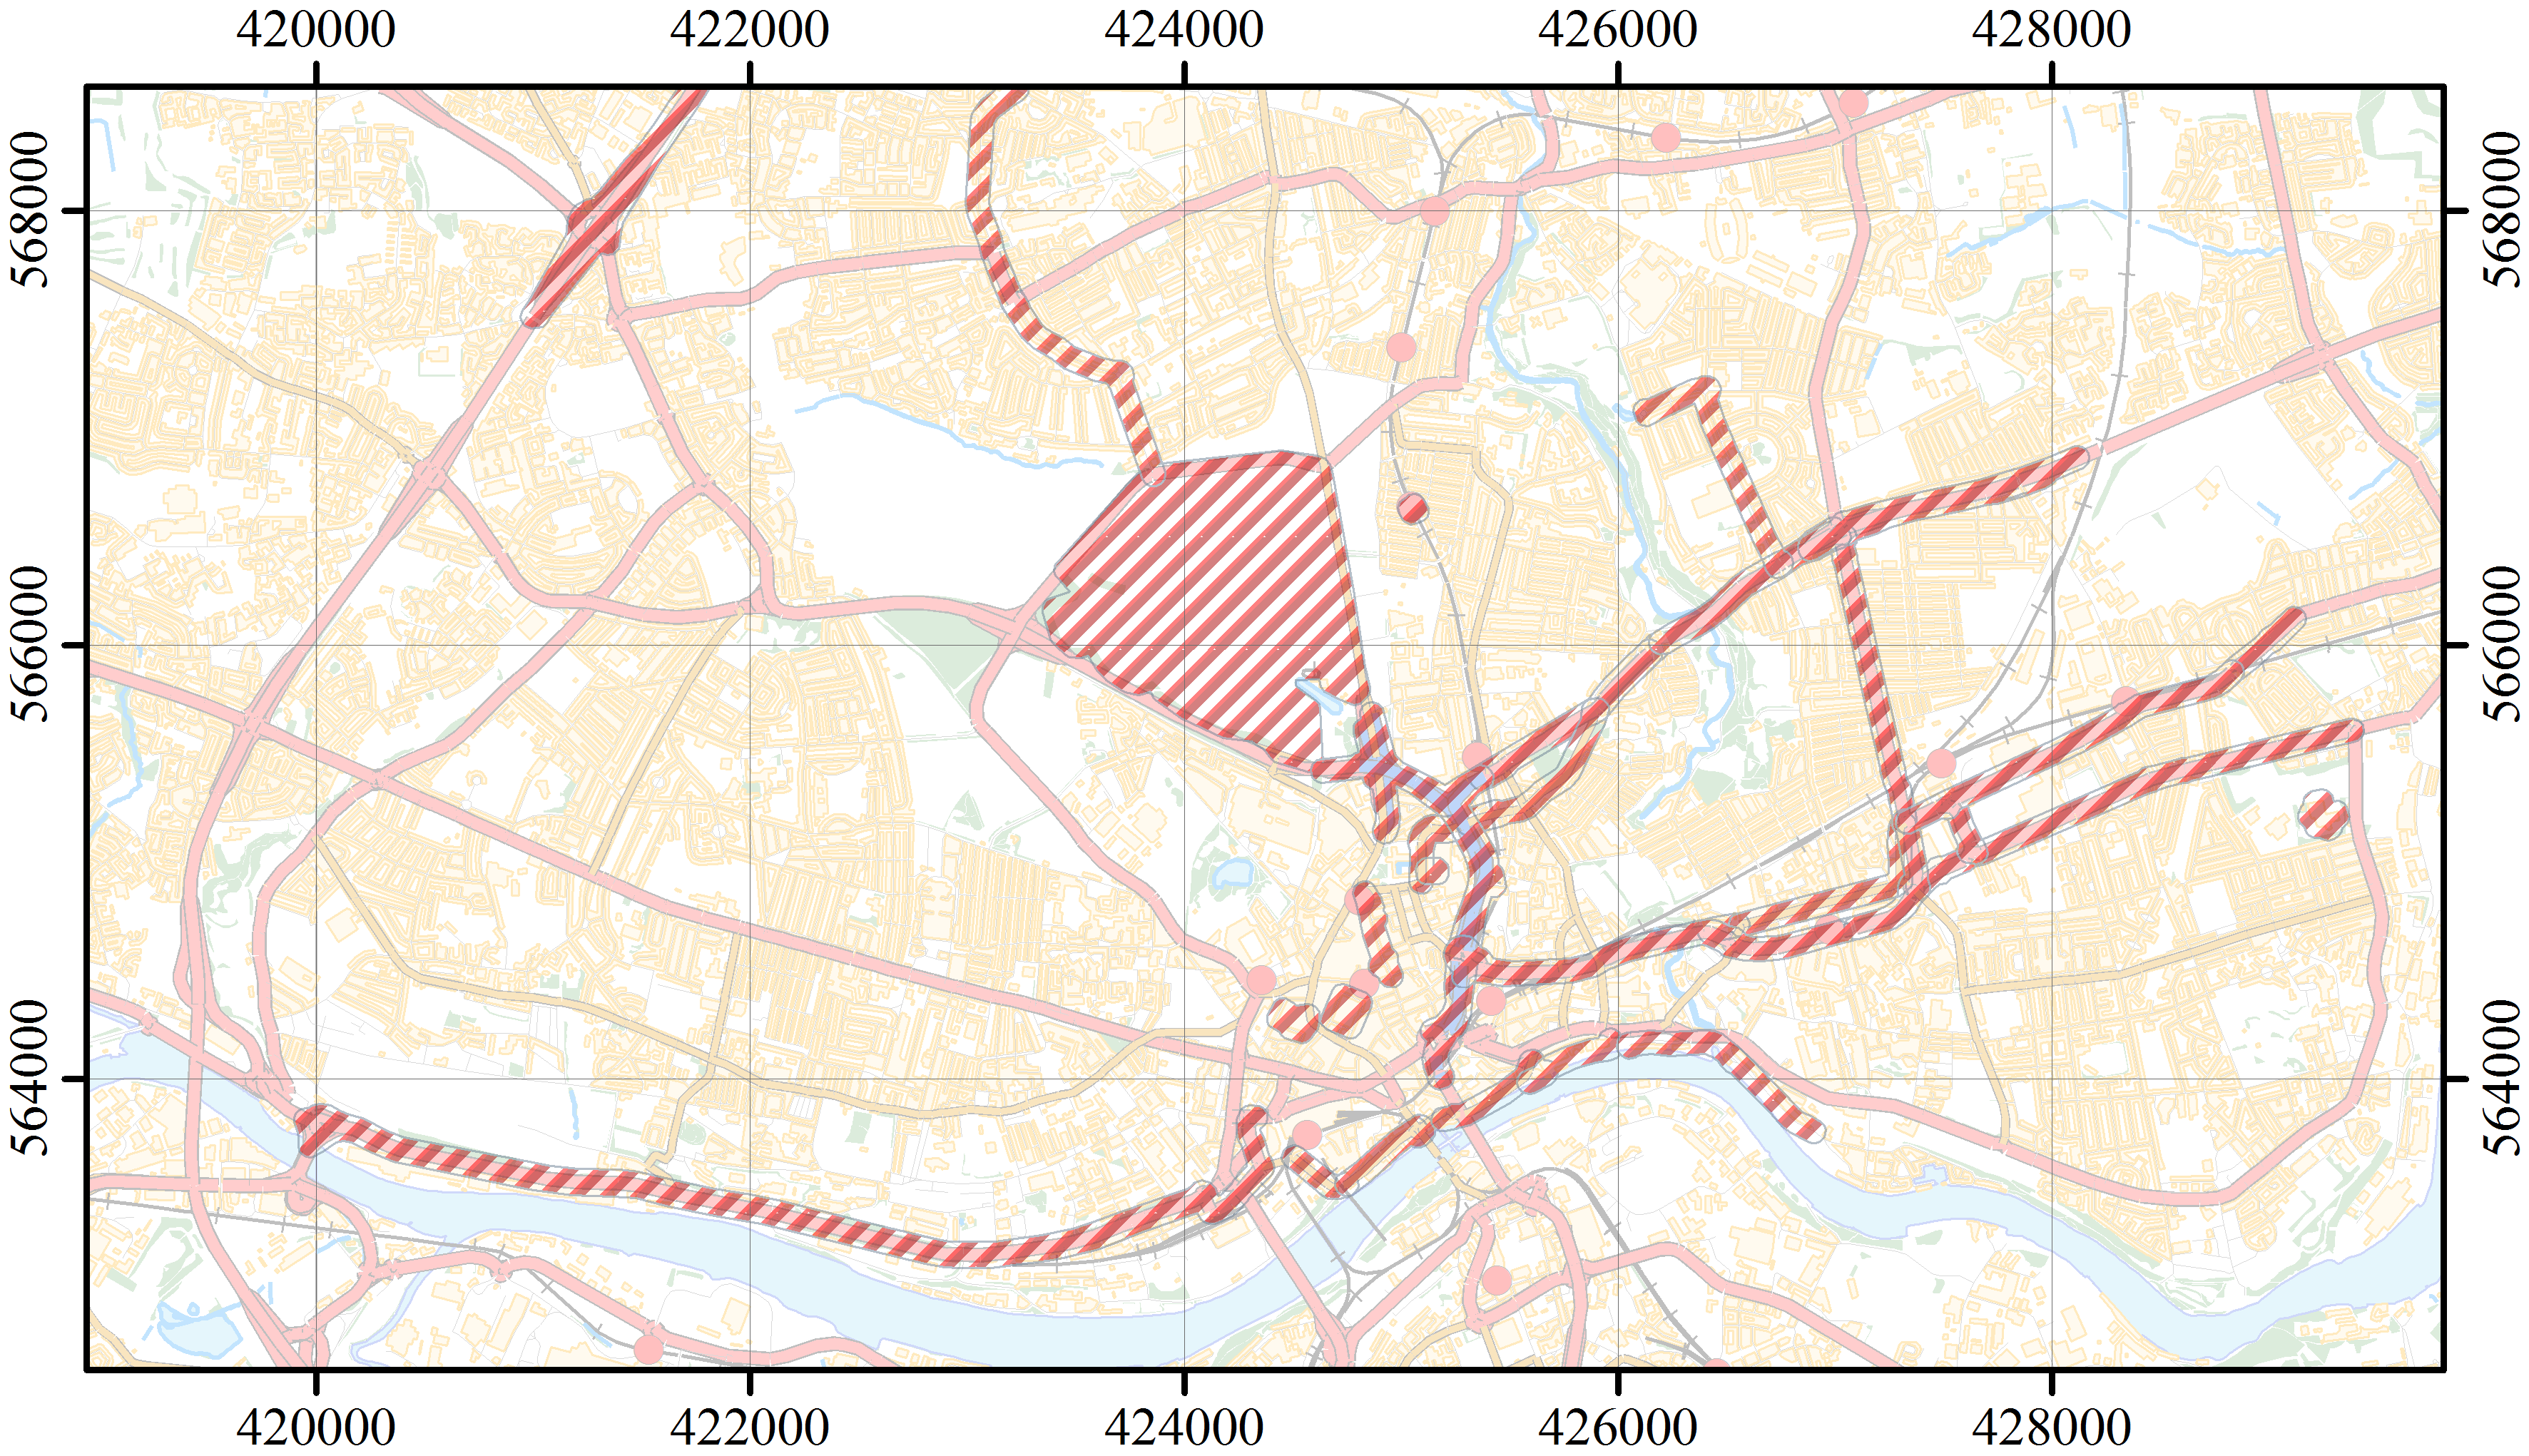
\includegraphics[width=1.0\textwidth]{nowcasting-figures/nclsm-identified-entities.png}
	\caption{Location of buffered spatial entities matched from Tweets.}
	\label{NclSM-Identified-Entities}
\end{figure*}

The majority of the locations matched were major roads in the city, as a consequence of these roads both being strategic routes affecting many people, and also the grade-separated junctions collecting water and quickly flooding, as shown in Figure \ref{NclSM-Identified-Entities}. Sometimes buildings were identified as flooding, which while useful information, the hydrodynamic model cannot reproduce flooding within the building as they are assumed to be solid. The models are likely to correctly reproduce internal flooding entering from the neighbouring streets through the depths in the buffered cells around a feature, but could not identify flooding as a result of leaking roofs. 

\subsection{Correlation of models against criteria from social media and known data}

Despite the low number of comparison criteria identified for the smaller 5th August event, a good match is easily identified, with the number of criteria satisfied reaching a plateau at approximately 30mm of rainfall, which is close to the actual amount, as shown in Figure \ref{NclSM-Percentage-Satisfied-5Aug}. No crowd-sourcing of photographic and textual data about the August event was undertaken, so there is little data to use for further validation.

\begin{figure*}[tpb]
	\centering
	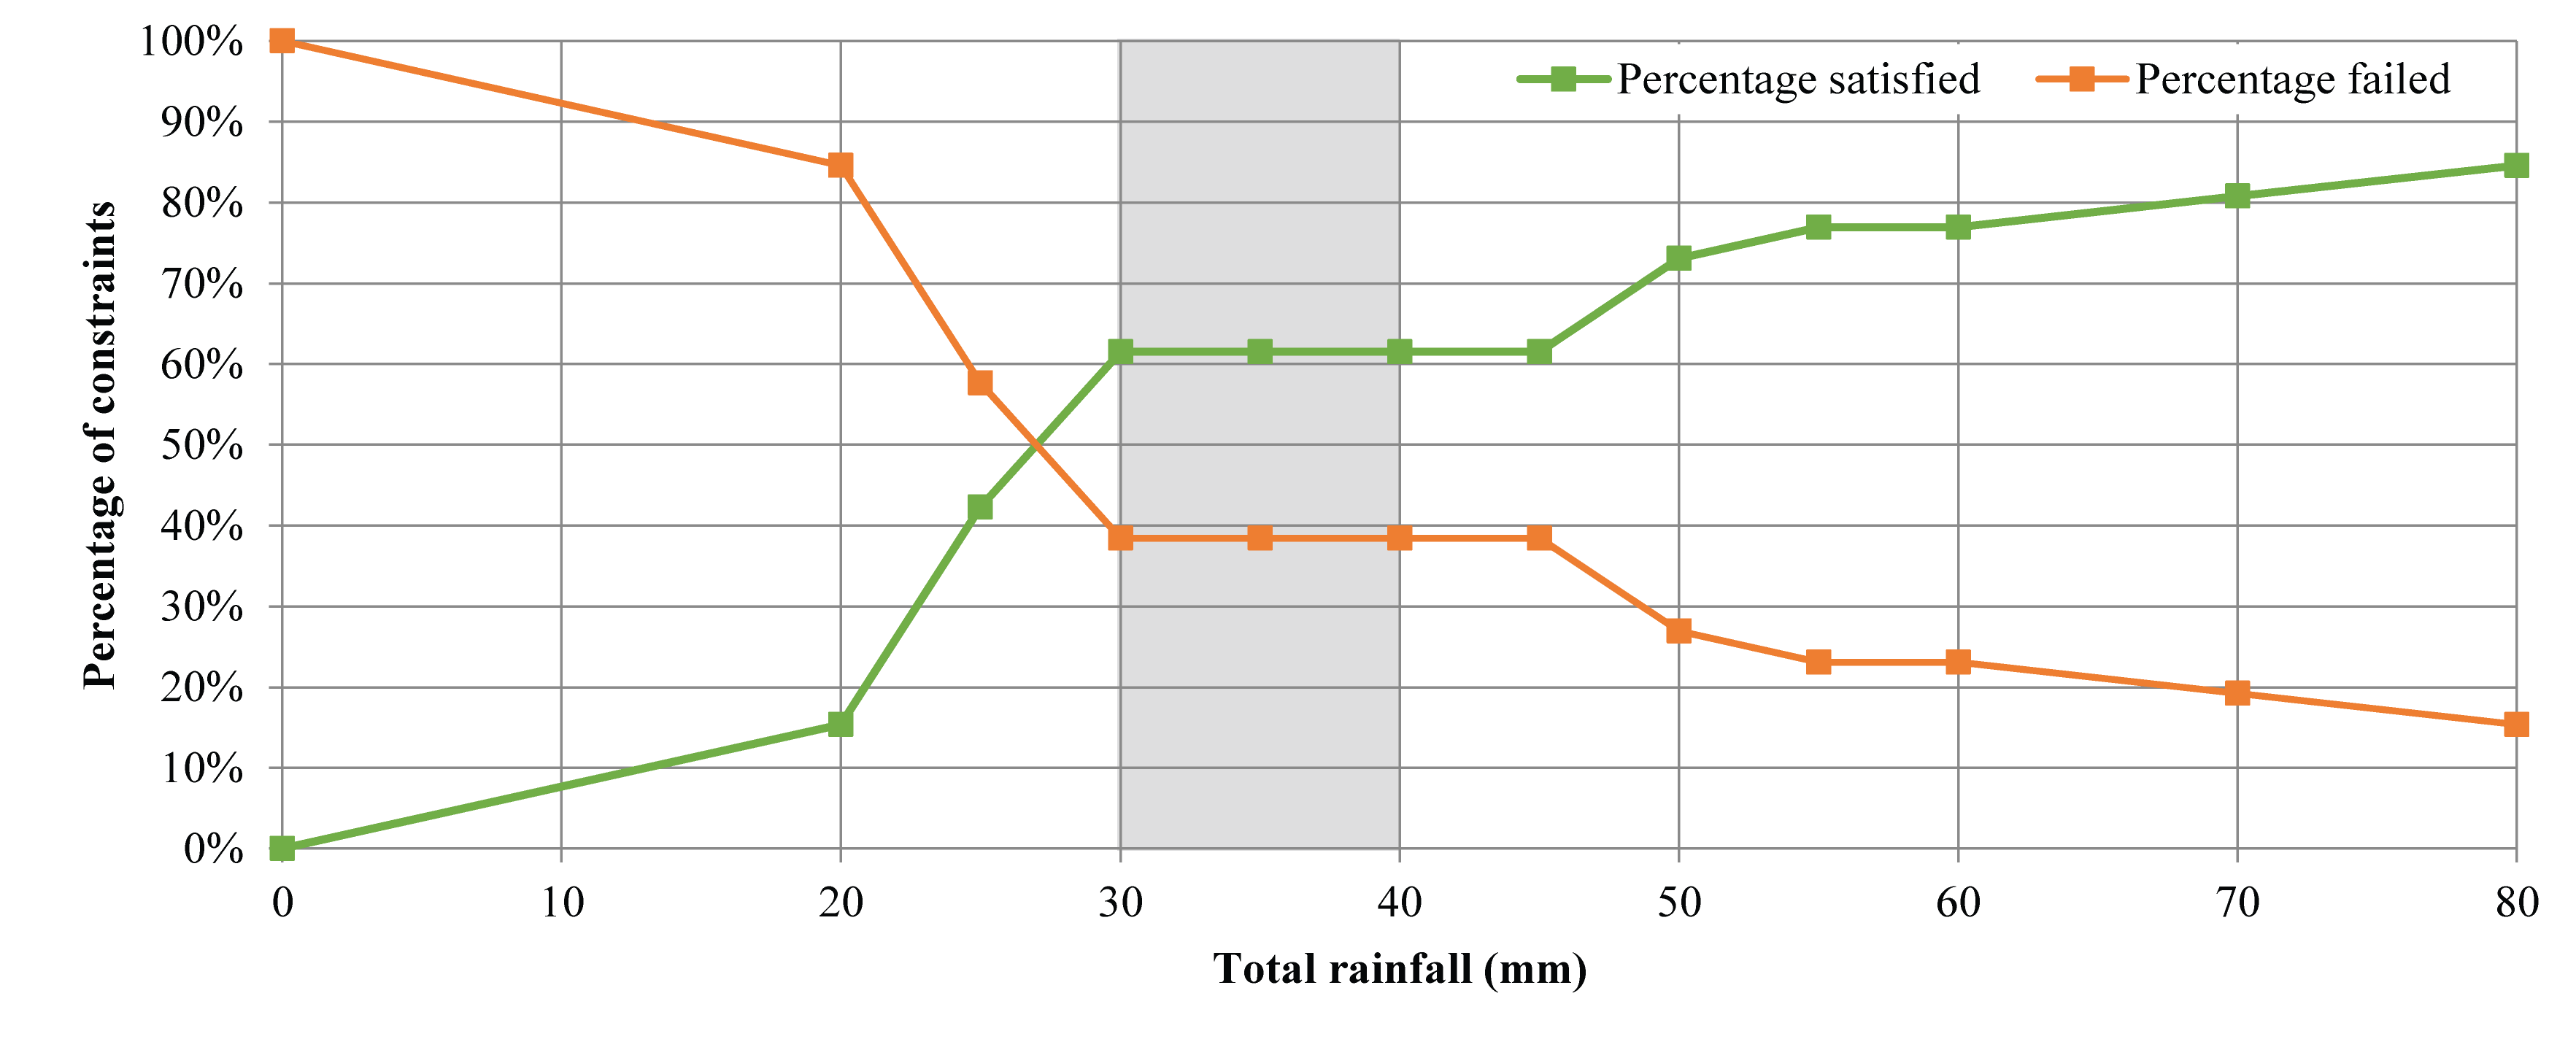
\includegraphics[width=1.0\textwidth]{nowcasting-figures/nclsm-percentage-satisfied-5aug.png}
	\caption{Percentage of model criteria from social media satisfied by different total rainfall amounts for the 5th August event.}
	\label{NclSM-Percentage-Satisfied-5Aug}
\end{figure*}

A greater volume of validation data is available for 28th June. The change in criteria satisfied becomes less than 5\% at 45mm of rainfall; however, as can be seen in Figure \ref{NclSM-Percentage-Satisfied-28Jun} this is marginal, with the next increase (from 50 to 55mm) seen to increase by slightly over 5\%. This is not altogether surprising: the framework makes no allowance for the temporally varying intensity of rainfall, and it is known that on 28th June the heaviest rainfall was at the start of the event. Consequently, flood depths for areas that have small catchment areas, and flood first, were underestimated at least to begin with. The spatial variation in rainfall intensity is also difficult to assess, with only a handful of reliable rain gauges in the city, and inaccuracies in rainfall radar \citep{Wood2000}.

\begin{figure*}[tpb]
	\centering
	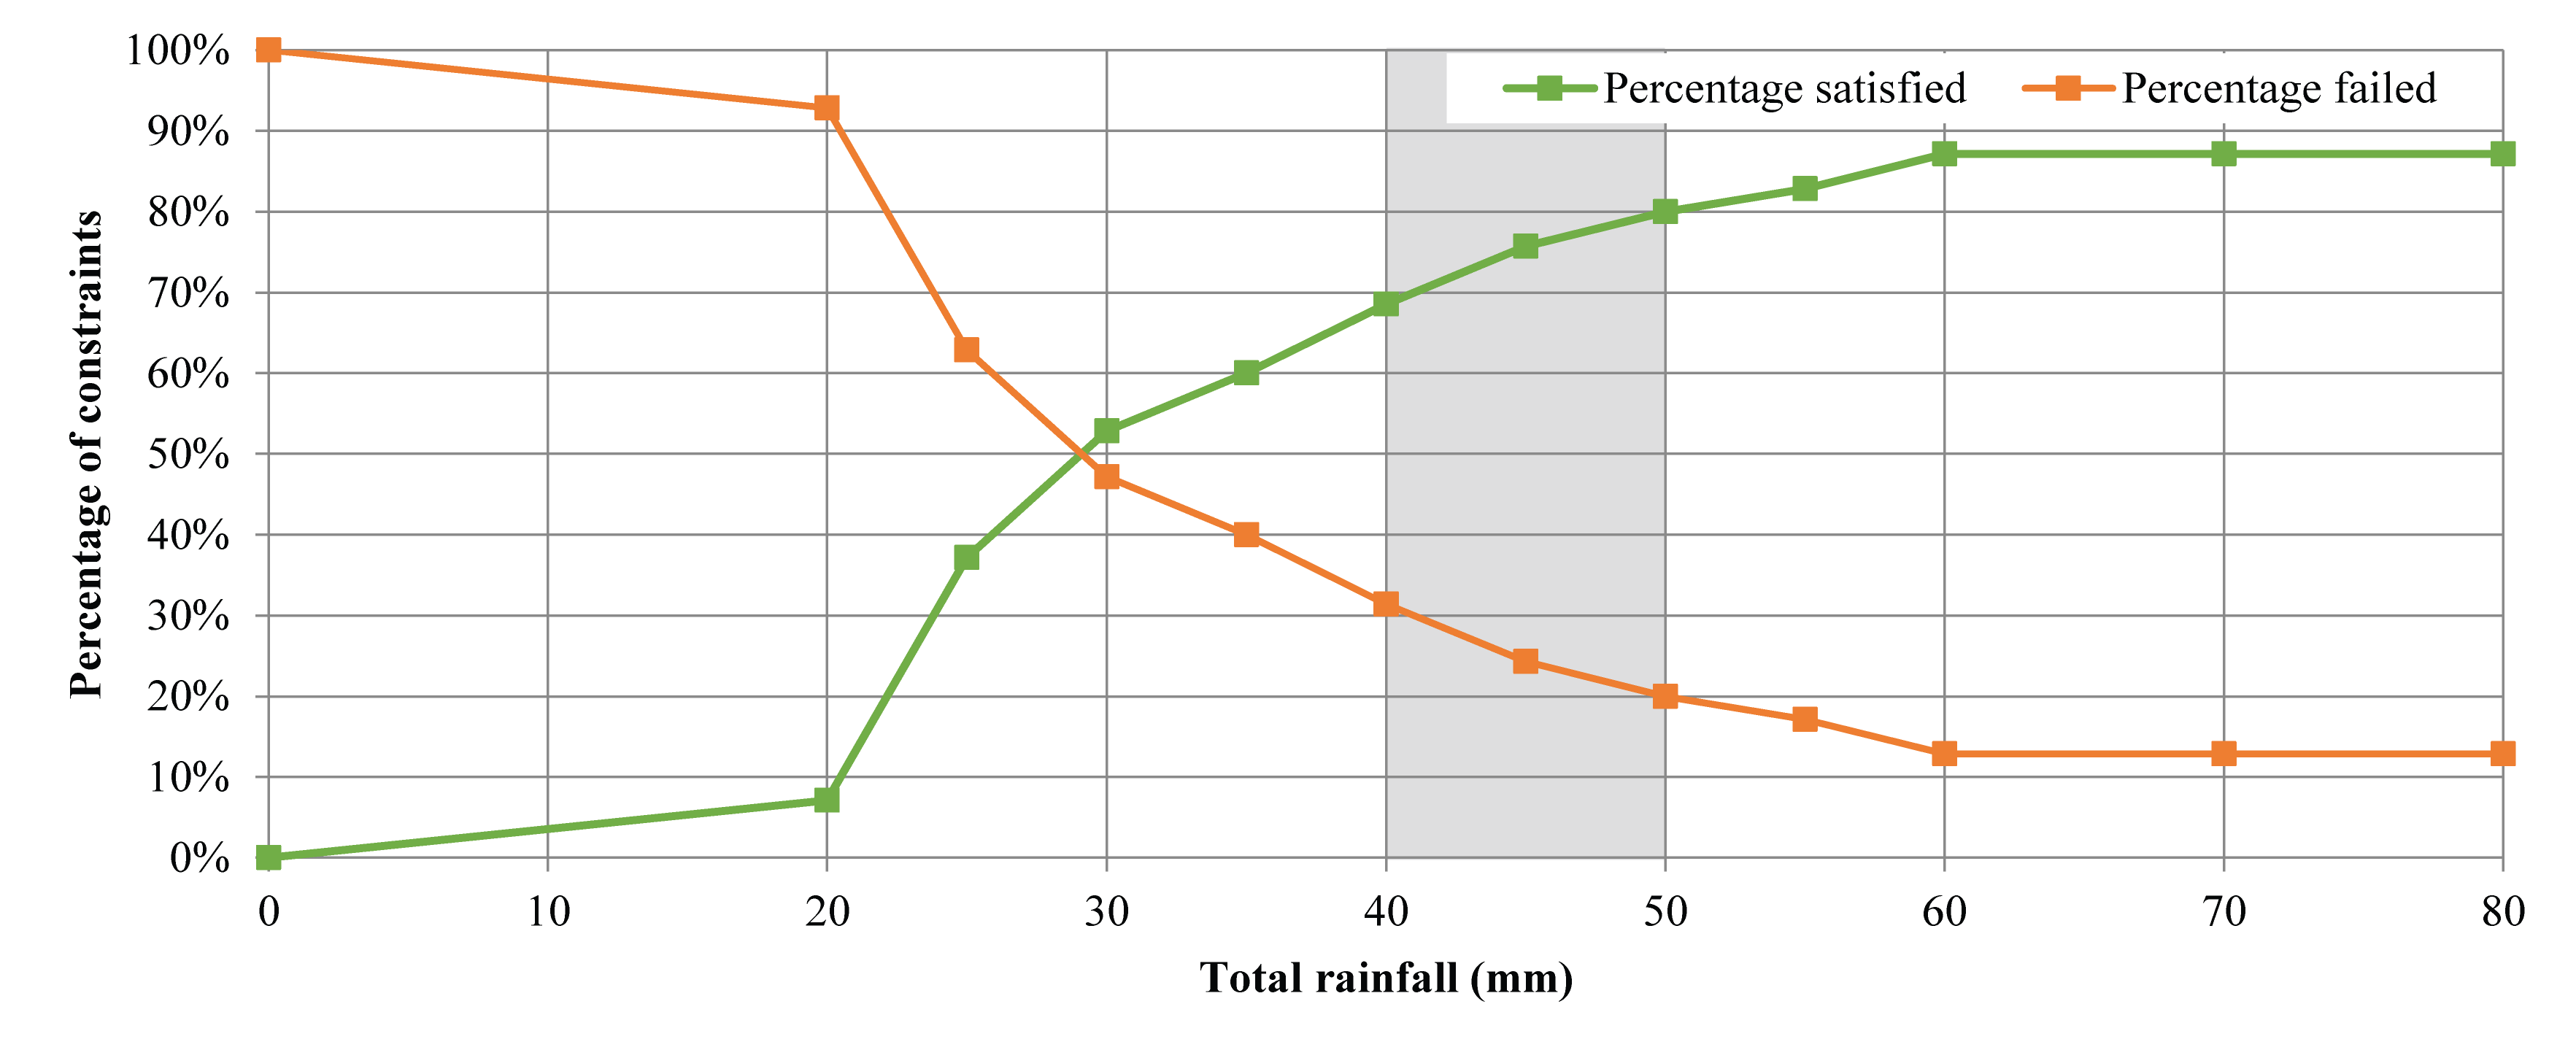
\includegraphics[width=1.0\textwidth]{nowcasting-figures/nclsm-percentage-satisfied-28jun.png}
	\caption{Percentage of model criteria from social media satisfied by different total rainfall amounts for the 28th June event.}
	\label{NclSM-Percentage-Satisfied-28Jun}
\end{figure*}

\begin{figure*}[tpb]
	\centering
	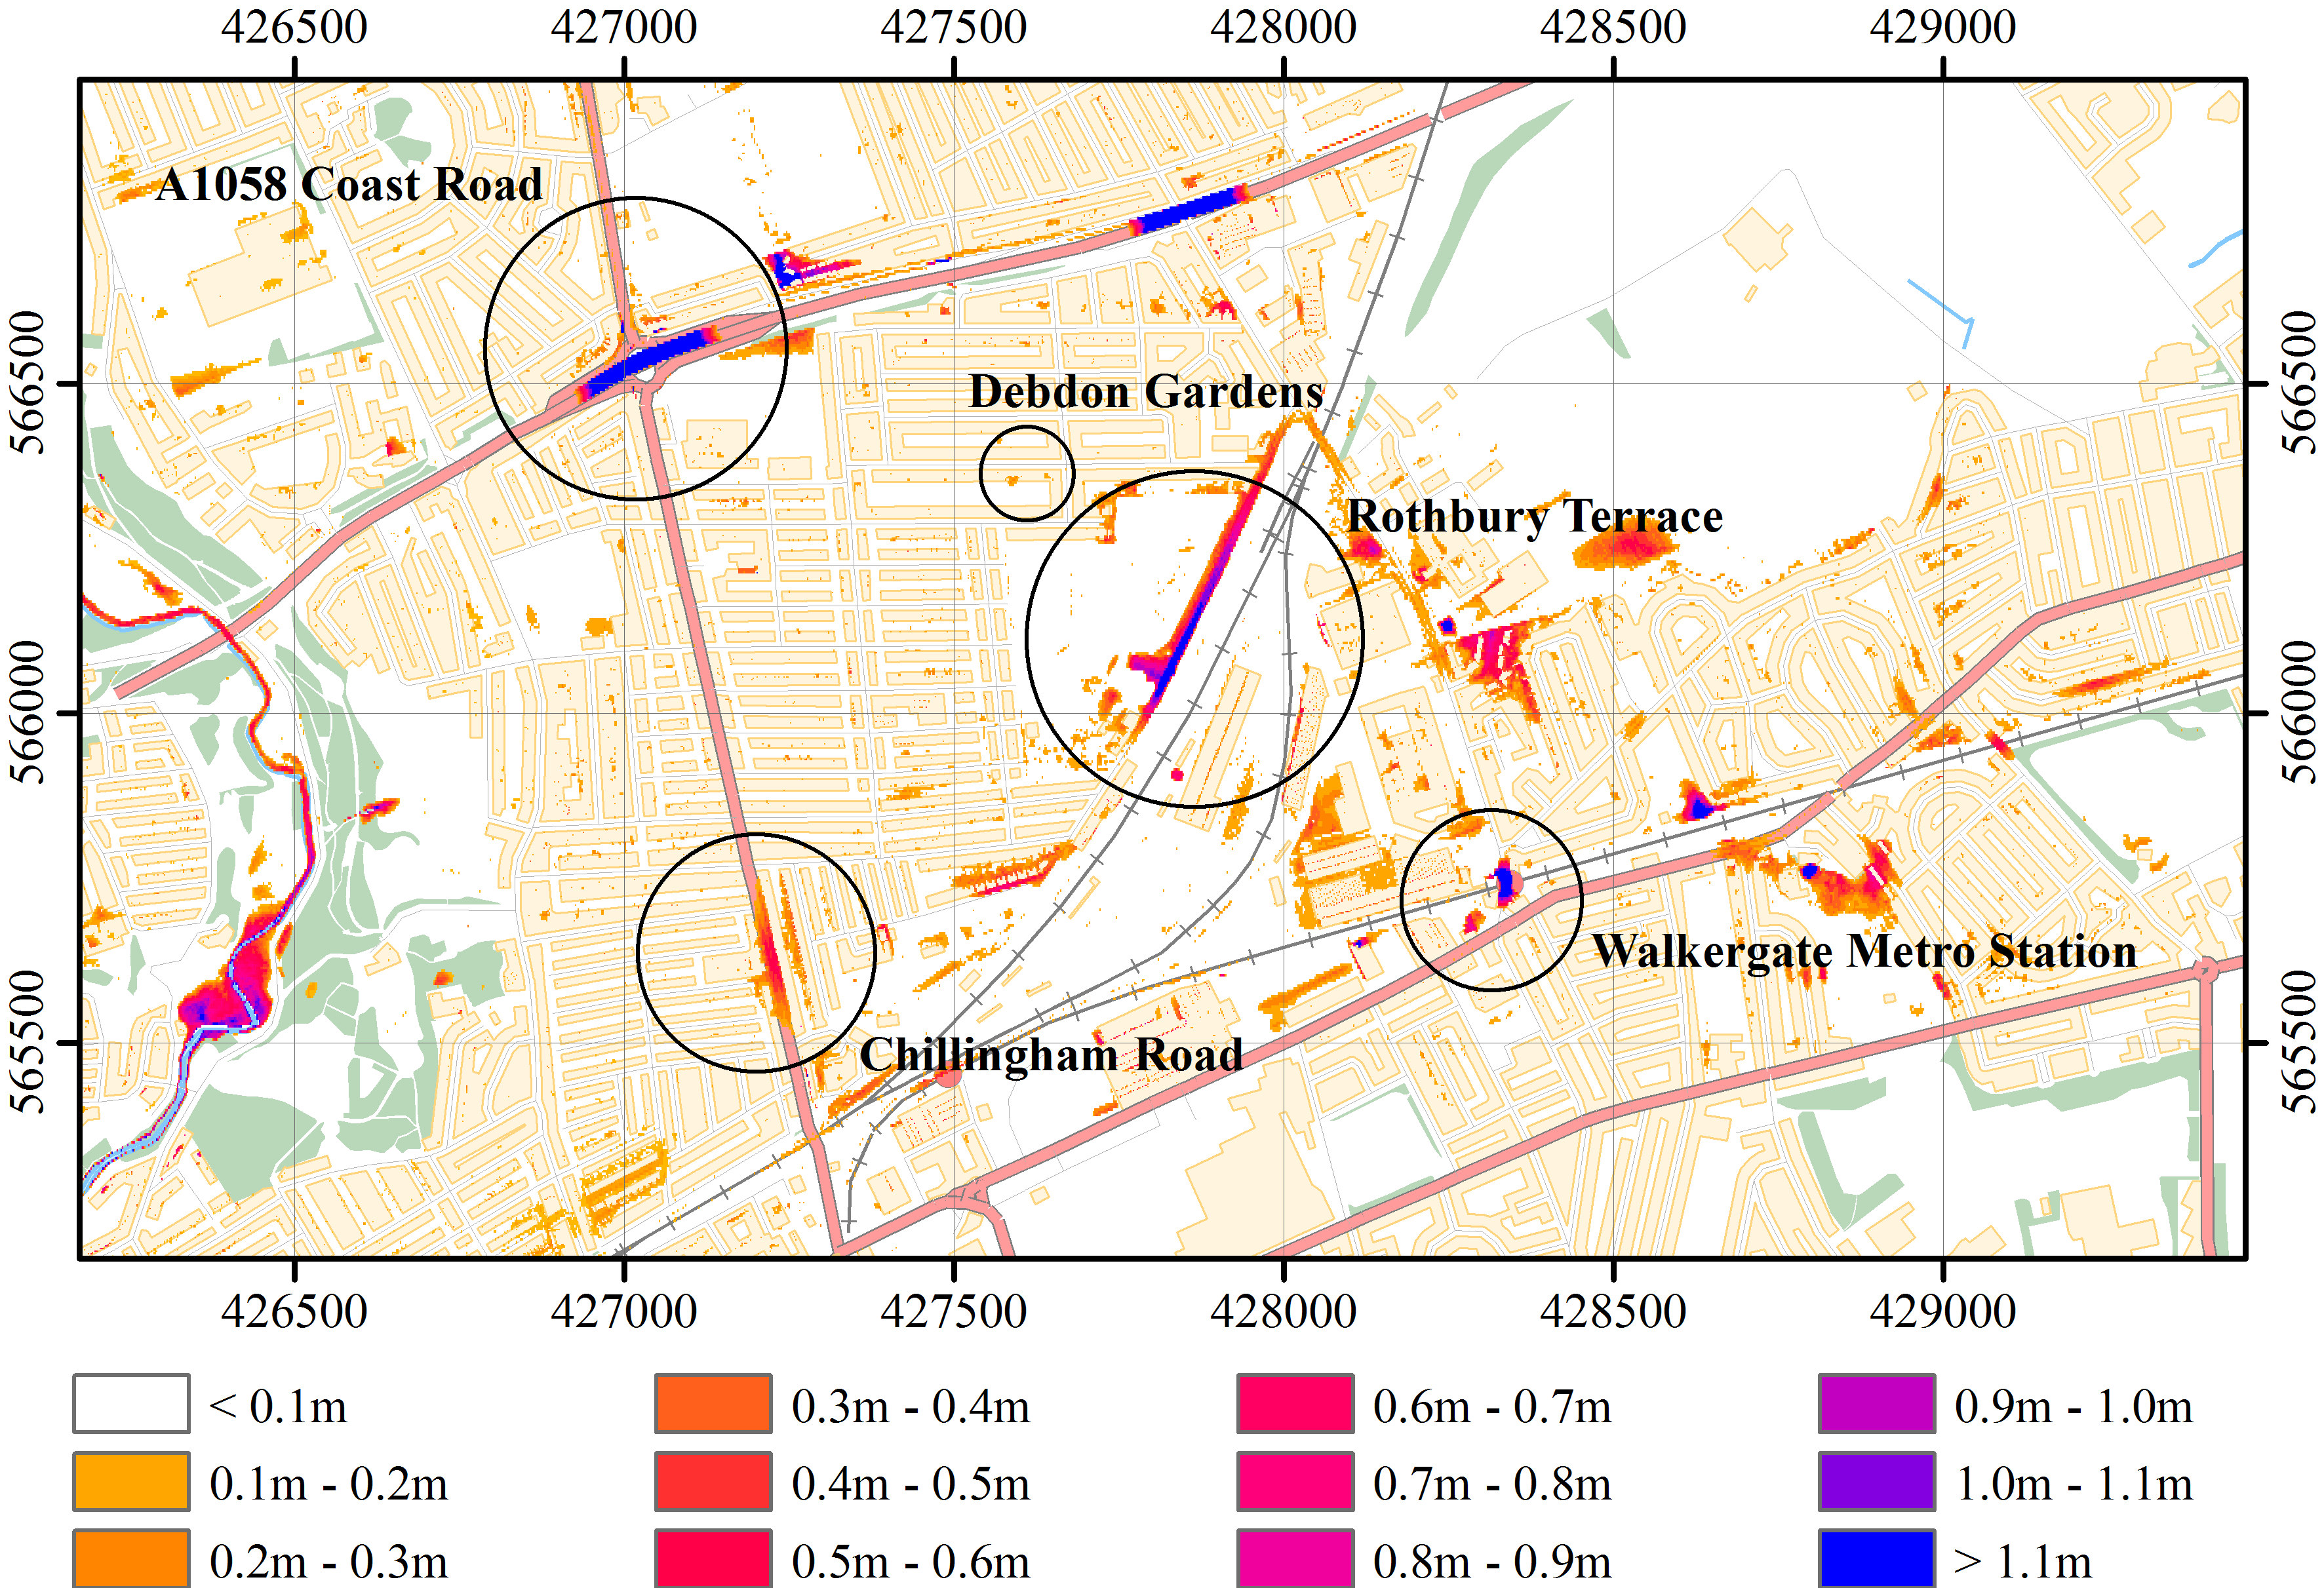
\includegraphics[width=1.0\textwidth]{nowcasting-figures/nclsm-depth-map.png}
	\caption{Flood depth map for 45mm of rainfall in the Heaton area of Newcastle upon Tyne, where circled areas correlate to areas known to have flooded from news reports and crowd-sourced photographs. Contains Ordnance Survey data \copyright{} Crown copyright and database right 2013.}
	\label{NclSM-Depth-Map}
\end{figure*}

Simulation results for 45mm to 60mm of rainfall all agree well with areas known to have flooded. A small area of the city is shown in Figure \ref{NclSM-Depth-Map} with areas known to have flooded highlighted. All of the circled areas except Debdon Gardens were identified as having flooded from Tweets, which in many cases included photos. The depths are a good approximate match against these photos. In the case of Debdon Gardens, crowd-sourced data from the public informed us that a small area of the road had flooded, with the water travelling through back gardens and collecting near the junction with Danby Gardens. Despite no social media data indicating the presence of flooding here, the simulation clearly shows a small area of flooding, with final depth approximately 0.25m. This clearly suggests that the framework is able to use areas with known flooding to automatically identify other areas likely to have flooded, in some cases at the level of individual properties. 

\section{Conclusions}

This chapter presented a framework for collecting and processing data about flooding in real-time during a storm event, which is used directly to instigate and evaluate computer simulations and extrapolate from the known extent to other areas likely to have flooded. The performance of the simulations when compared to data obtained through crowd-sourcing and from elsewhere, demonstrates that whilst the volume of rainfall cannot be determined exactly owing to other unknowns (e.g. the efficacy of the drainage network), the extent and depth of flooding is reproduced in most cases, even with small numbers of model criteria identified in social media. It is important to note that only two events are considered herein, and there is no guarantee of reproducibility, especially for areas with fewer social media users. With respect to the utility of social media in flood risk management, the evidence from Newcastle upon Tyne suggests that

\begin{enumerate}
	\item whilst there are data within Tweets regarding the location of flooding, indications of depth are often absent, and the associated timestamp may not be representative of the observation;
	\item initial activity on social media tends to focus on the intensity of the weather, whilst useful activity detailing areas explicitly affected can sometimes come much later;
	\item a considerable number of useful data identified was distributed by local authorities, emergency responders, and other public sector organisations, based on reports from the public made by other means and CCTV cameras; and
	\item photographs have value for retrospective analysis of an event, but social media sites generally strip embedded data including the date and time of capture, hence other means of collecting photographs which preserve this information may be required.
\end{enumerate}

Potential avenues for improving the framework have been identified, primarily focusing on improved interpretation of Tweets and matching ambiguous terms. The framework is clearly better suited to incident management applications than forecasting, but provides a basis through which the public can be informed of the best routes for travelling, and local authorities can identify the areas requiring the most immediate attention. 